\documentclass{LMCS}

\def\dOi{10(1:16)2014}
\lmcsheading {\dOi}
{1--42}
{}
{}
{Mar.~\phantom04, 2013}
{Mar.~\phantom03, 2014}
{}

\subjclass{Models of Computation, Probabilistic Computation,
  Concurrency, Process Calculi}

\ACMCCS{[{\bf Theory of computation}]: Models of
  Computation---Probabilistic Computation;  Models of
  computation---Concurrency---Process calculi} 

\usepackage{amsmath,amsfonts,amstext,amssymb,mathrsfs,stmaryrd}
\usepackage{latexsym}
\usepackage{graphicx}
\usepackage{color}
\usepackage{proof}
\usepackage{hyperref}


\def\ms#1{\null\ifmmode\mathord{\mathcode`-="702D\it #1\mathcode`\-="2200}\else\fi}

\newcommand{\cws}[2]
	{\\ \centerline{} \0.5cm]
& \!\!\! = \!\!\! & a. (\sum\limits_{s' \in \ms{supp}(\cald')} \, \sum\limits_{s'_0 \in \ms{supp}(\cald'')}
(\cald'(s') \cdot \ms{traces}_{j}(s')) \otimes_{\cala} (\cald''(s'_0) \cdot \ms{traces}_{h}(s'_0)))
\0.5cm]
& \!\!\! = \!\!\! & a. (\sum\limits_{s' \in \ms{supp}(\cald')} \cald'(s') \cdot \ms{traces}_{j}(s'))
\otimes_{\cala} a. (\sum\limits_{s'_0 \in \ms{supp}(\cald'')} \cald''(s'_0) \cdot \ms{traces}_{h}(s'_0))
\0.5cm]
& & a. (\sum\limits_{s'_0 \in \ms{supp}(\cald'')} \cald''(s'_0) \cdot (\ms{traces}_{j}(s) \otimes_{\cala}
\ms{traces}_{h}(s'_0))) \0.5cm]
& & a. (\ms{traces}_{j}(s) \otimes_{\cala} (\sum\limits_{s'_0 \in \ms{supp}(\cald'')} \cald''(s'_0) \cdot
\ms{traces}_{h}(s'_0))) \0.5cm]
& & \ms{traces}_{j}(s) \otimes_{\cala} (a. (\sum\limits_{s'_0 \in \ms{supp}(\cald'')} \cald''(s'_0) \cdot
\ms{traces}_{h}(s'_0))) \0.4cm]
\bigsqcap\limits_{\calz_{1} \in \ms{Res}_{\rm max}(s_{1}, o)} \ms{prob}(\calsc(z_{s_{1}, o})) & \!\!\! =
\!\!\! & \bigsqcap\limits_{\calz_{2} \in \ms{Res}_{\rm max}(s_{2}, o)} \ms{prob}(\calsc(z_{s_{2}, o})) \\
\end{array}}
We denote by  the variant based on randomized schedulers.
\fullbox

	\end{defi}

Following the structure of classical testing equivalence  for fully nondeterministic
processes~\cite{DH84}, the constraint on suprema represents the may-part of
 while the constraint on infima represents the must-part of
. The probabilistic testing equivalences in~\cite{YL92,JY95,DGHM08} are
essentially defined as , while the one in~\cite{Seg96} resolves
nondeterminism through randomized schedulers instead of deterministic ones and makes use of countably many
success actions in place of a single one. Notably, a single success action suffices when testing finitary
processes, as proved in~\cite{DGMZ07}, and the use of different classes of schedulers does not change the
discriminating power, as we now show.

	\begin{thm}\label{thm:ptesupinf_sched}

Let  be an NPLTS and . Then:
\cws{12}{s_{1} \sbis{\textrm{{\rm PTe}-}\sqcup\sqcap}^{\rm ct} s_{2} \: \Longleftrightarrow \: s_{1}
\sbis{\textrm{{\rm PTe}-}\sqcup\sqcap} s_{2}}

\proof
The result follows from the fact that, given an arbitrary state  and an arbitrary NPT  with initial state , it holds that:
\cws{0}{\begin{array}{rcl}
\bigsqcup\limits_{\calz \in \ms{Res}^{\rm ct}_{\rm max}(s, o)} \ms{prob}(\calsc(z_{s, o})) & \!\!\! = \!\!\!
& \bigsqcup\limits_{\calz \in \ms{Res}_{\rm max}(s, o)} \ms{prob}(\calsc(z_{s, o})) \0.6cm]
\hspace*{0.4cm} = \: \bigsqcup\limits_{\calz \in \ms{Res}_{\rm max}(s, o)} \hspace{-0.7cm}
\ms{prob}(\calsc(z_{s, o})) \\
\end{array}}
where in the third line we have exploited the induction hypothesis and in the seventh line the fact that
.
\qed 

		\end{itemize}

	\end{thm}

The relation  does not enjoy the desirable property -- possessed by
 -- of resulting in a testing semantics finer than the trace semantics for the same class
of processes. Whether  is included in the trace equivalences of
Sect.~\ref{sec:trace_equiv} depends on the type of schedulers that are considered on the trace semantics
side. In the case of randomized schedulers, as shown in~\cite{Seg96} it holds that
, and hence
 by virtue of
Thm.~\ref{thm:ptrdis_incl_ptr}. However, inclusion no longer holds when only deterministic schedulers are
admitted. Let us consider the two NPLTS models in Fig.~\ref{fig:counterex_ptesupinf_trace}. We have that
 while  and . It holds that  because, for any
test, the central maximal resolution of  always gives rise to a success probability comprised between
the success probabilities of the other two maximal resolutions of , which correspond to the two
maximal resolutions of . In contrast,  and  are not related by the two probabilistic
trace equivalences because the maximal resolution of  starting with the central -transition is not
matched by any of the two maximal resolutions of .

	\begin{figure}[tp]

	\begin{center}

	\begin{tabular}{c@{\hspace{2.5cm}}c}

	\ifwithtikz
\tikzsetnextfilename{counterex_ptesupinf_trace_a}
	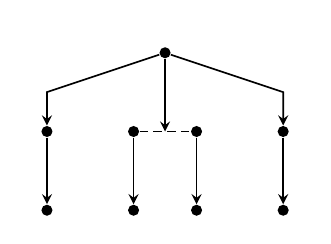
\begin{tikzpicture}[
		every label/.style={font=\scriptsize},
		state/.style={inner sep=0pt,fill,minimum size=4pt,circle,font=\scriptsize},
		arc/.style={->,>=stealth,semithick},
		probability/.style={-,densely dashed},
	]

\node [state,label=] (s2) at (1.5,1.0) {};	

\node [inner sep=0pt,circle,fill,minimum size=4pt] (s2_1) at (0.0,0.0) {};
\node [inner sep=0pt,circle,fill,minimum size=4pt,label=] (s2_2) at (1.1,0.0) {};
\node [inner sep=0pt,circle,fill,minimum size=4pt,label=] (s2_3) at (1.9,0.0) {};
\node [inner sep=0pt,circle,fill,minimum size=4pt] (s2_4) at (3,0.0) {};

\node [inner sep=0pt,circle,fill,minimum size=4pt] (s2_5) at (0.0,-1.0) {};
\node [inner sep=0pt,circle,fill,minimum size=4pt] (s2_6) at (1.1,-1.0) {};
\node [inner sep=0pt,circle,fill,minimum size=4pt] (s2_7) at (1.9,-1.0) {};
\node [inner sep=0pt,circle,fill,minimum size=4pt] (s2_8) at (3.0,-1.0) {};

\draw [arc] (s2) to (0.0,0.5) to node [auto,pos=-0.2,swap,font=\scriptsize] {}  (s2_1);
\draw [arc] (s2) to node [auto,pos=0.35,swap,font=\scriptsize] {} (1.5,0.0);
\draw [arc] (s2) to (3.0,0.5) to node [auto,pos=-0.2,font=\scriptsize] {} (s2_4);

\draw [probability] (s2_2) -- (s2_3);

\draw [arc] (s2_1) to node [auto,swap,font=\scriptsize,anchor=base east] {}  (s2_5);
\draw [arc] (s2_2) to node [auto,swap,font=\scriptsize,anchor=base east] {}  (s2_6);
\draw [arc] (s2_3) to node [auto,font=\scriptsize,anchor=base west] {}  (s2_7);
\draw [arc] (s2_4) to node [auto,font=\scriptsize,anchor=base west] {}  (s2_8);
	
	\end{tikzpicture}	
	\else
	\includegraphics{Pictures/counterex_ptesupinf_trace_a}
	\fi
	
	&

	\ifwithtikz
\tikzsetnextfilename{counterex_ptesupinf_trace_b}
	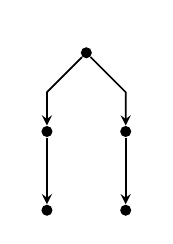
\begin{tikzpicture}[
		every label/.style={font=\scriptsize},
		state/.style={inner sep=0pt,fill,minimum size=4pt,circle,font=\scriptsize},
		arc/.style={->,>=stealth,semithick},
		probability/.style={-,densely dashed},
	]

\node [state,label=] (s2) at (1.5,1.0) {};	

\node [inner sep=0pt,circle,fill,minimum size=4pt] (s2_1) at (1.0,0.0) {};
\node [inner sep=0pt,circle,fill,minimum size=4pt] (s2_4) at (2.0,0.0) {};

\node [inner sep=0pt,circle,fill,minimum size=4pt] (s2_5) at (1.0,-1.0) {};
\node [inner sep=0pt,circle,fill,minimum size=4pt] (s2_8) at (2.0,-1.0) {};

\draw [arc] (s2) to (1.0,0.5) to node [auto,pos=-0.2,swap,font=\scriptsize] {} (s2_1);
\draw [arc] (s2) to (2.0,0.5) to node [auto,pos=-0.2,font=\scriptsize] {}  (s2_4);

\draw [arc] (s2_1) to node [auto,swap,font=\scriptsize,anchor=base east] {}  (s2_5);
\draw [arc] (s2_4) to node [auto,font=\scriptsize,anchor=base west] {}  (s2_8);
	
	\end{tikzpicture}	
	\else
	\includegraphics{Pictures/counterex_ptesupinf_trace_b}
	\fi
	
	\end{tabular}

	\end{center}
 \caption{NPLTS models identified by / and
told apart by /}
\label{fig:counterex_ptesupinf_trace}

	\end{figure}

Under deterministic schedulers, inclusion can be achieved by considering  in lieu of the
finer  and the new testing equivalence  introduced
by the next definition in lieu of the coarser~. Instead of focussing only
on extremal success probabilities,  requires matching the success
probabilities of \emph{all} maximal resolutions of the interaction systems. Interestingly, the variant of
 based on randomized schedulers coincides with
.

	\begin{defi}\label{def:pteallexists}

Let  be an NPLTS. We say that  are \emph{probabilistic
-testing equivalent}, written , iff for
every NPT  with initial state  it holds that:

		\begin{itemize}

\item For each  there exists  such that:
\cws{10}{\hspace*{-1.2cm} \ms{prob}(\calsc(z_{s_{1}, o})) \: = \: \ms{prob}(\calsc(z_{s_{2}, o}))}

\item For each  there exists  such that:
\cws{10}{\hspace*{-1.2cm} \ms{prob}(\calsc(z_{s_{2}, o})) \: = \: \ms{prob}(\calsc(z_{s_{1}, o}))}

		\end{itemize}

\noindent
We denote by  the coarser variant based on randomized
schedulers.
\fullbox

	\end{defi}

	\begin{figure}[tp]

	\begin{center}

	\begin{tabular}{c@{\hspace{.5cm}}c@{\hspace{.5cm}}c}
	\ifwithtikz
\tikzsetnextfilename{test_pteallexists_a}
	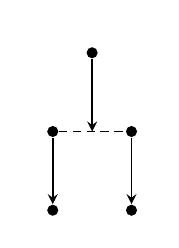
\begin{tikzpicture}[
		every label/.style={font=\scriptsize},
		state/.style={inner sep=0pt,fill,minimum size=4pt,circle,font=\scriptsize},
		arc/.style={->,>=stealth,semithick},
		probability/.style={-,densely dashed},
	]

\node [state,label=] (s2) at (1.5,1.0) {};	

\node [inner sep=0pt,circle,fill,minimum size=4pt,label=] (s2_1) at (1.0,0.0) {};
\node [inner sep=0pt,circle,fill,minimum size=4pt,label=] (s2_4) at (2.0,0.0) {};

\node [inner sep=0pt,circle,fill,minimum size=4pt,label=left:] (s2_5) at (1.0,-1.0) {};
\node [inner sep=0pt,circle,fill,minimum size=4pt] (s2_8) at (2.0,-1.0) {};

\draw [arc] (s2) to node [auto,pos=0.35,swap,font=\scriptsize] {} (1.5,0.0);

\draw [probability] (s2_1) -- (s2_4);

\draw [arc] (s2_1) to node [auto,swap,font=\scriptsize,anchor=base east] {}  (s2_5);
\draw [arc] (s2_4) to node [auto,font=\scriptsize,anchor=base west] {}  (s2_8);
	
	\end{tikzpicture}
	\else
	
	\includegraphics{Pictures/test_pteallexists_a}
	
	\fi	

	&

	\ifwithtikz
\tikzsetnextfilename{test_pteallexists_b}
	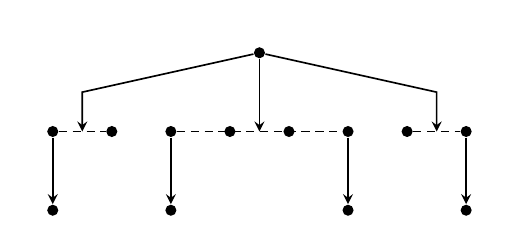
\begin{tikzpicture}[
		every label/.style={font=\scriptsize},
		state/.style={inner sep=0pt,fill,minimum size=4pt,circle,font=\scriptsize},
		arc/.style={->,>=stealth,semithick},
		probability/.style={-,densely dashed},
	]

\node [state,label={}] (s1) at (2.625,1.0) {};	

\node [inner sep=0pt,circle,fill,minimum size=4pt,label=] (s1_1) at (0.0,0.0) {};
\node [inner sep=0pt,circle,fill,minimum size=4pt,label=] (s1_2) at (0.75,0.0) {};
\node [inner sep=0pt,circle,fill,minimum size=4pt,label=] (s1_3) at (1.5,0.0) {};
\node [inner sep=0pt,circle,fill,minimum size=4pt,label=] (s1_4) at (2.25,0.0) {};
\node [inner sep=0pt,circle,fill,minimum size=4pt,label=] (s1_5) at (3.0,0.0) {};
\node [inner sep=0pt,circle,fill,minimum size=4pt,label=] (s1_6) at (3.75,0.0) {};
\node [inner sep=0pt,circle,fill,minimum size=4pt,label=] (s1_7) at (4.5,0.0) {};
\node [inner sep=0pt,circle,fill,minimum size=4pt,label=] (s1_8) at (5.25,0.0) {};

\node [inner sep=0pt,circle,fill,minimum size=4pt,label=left:] (s1_9) at (0.0,-1.0) {};
\node [inner sep=0pt,circle,fill,minimum size=4pt,label=left:] (s1_10) at (1.5,-1.0) {};
\node [inner sep=0pt,circle,fill,minimum size=4pt] (s1_11) at (3.75,-1.0) {};
\node [inner sep=0pt,circle,fill,minimum size=4pt] (s1_12) at (5.25,-1.0) {};

\draw [arc] (s1) to (0.375,0.5) to node [auto,pos=-0.2,swap,font=\scriptsize] {} (0.375,0.0);
\draw [arc] (s1) to node [auto,pos=0.35,swap,font=\scriptsize] {} (2.625,0.0);
\draw [arc] (s1) to (4.875,0.5) to node [auto,pos=-0.2,font=\scriptsize] {} (4.875,0.0);

\draw [probability] (s1_1) -- (s1_2);
\draw [probability] (s1_3) -- (s1_6);
\draw [probability] (s1_7) -- (s1_8);
\draw [arc] (s1_1) to node [auto,swap,font=\scriptsize,anchor=base east] {}  (s1_9);
\draw [arc] (s1_3) to node [auto,swap,font=\scriptsize,anchor=base east] {}  (s1_10);
\draw [arc] (s1_6) to node [auto,font=\scriptsize,anchor=base west] {}  (s1_11);
\draw [arc] (s1_8) to node [auto,font=\scriptsize,anchor=base west] {}  (s1_12);
	
	\end{tikzpicture}	
	\else
	
	\includegraphics{Pictures/test_pteallexists_b}
	
	\fi
	
&

	\ifwithtikz
\tikzsetnextfilename{test_pteallexists_c}
	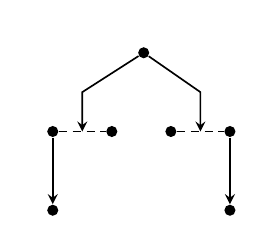
\begin{tikzpicture}[
		every label/.style={font=\scriptsize},
		state/.style={inner sep=0pt,fill,minimum size=4pt,circle,font=\scriptsize},
		arc/.style={->,>=stealth,semithick},
		probability/.style={-,densely dashed},
	]

\node [state,label={}] (s1) at (1.155,1.0) {};	

\node [inner sep=0pt,circle,fill,minimum size=4pt,label=] (s1_1) at (0.0,0.0) {};
\node [inner sep=0pt,circle,fill,minimum size=4pt,label=] (s1_2) at (0.75,0.0) {};
\node [inner sep=0pt,circle,fill,minimum size=4pt,label=] (s1_7) at (1.5,0.0) {};
\node [inner sep=0pt,circle,fill,minimum size=4pt,label=] (s1_8) at (2.25,0.0) {};

\node [inner sep=0pt,circle,fill,minimum size=4pt,label=left:] (s1_9) at (0.0,-1.0) {};
\node [inner sep=0pt,circle,fill,minimum size=4pt] (s1_12) at (2.25,-1.0) {};

\draw [arc] (s1) to (0.375,0.5) to node [auto,pos=-0.2,swap,font=\scriptsize] {} (0.375,0.0);
\draw [arc] (s1) to (1.875,0.5) to node [auto,pos=-0.2,font=\scriptsize] {} (1.875,0.0);

\draw [probability] (s1_1) -- (s1_2);
\draw [probability] (s1_7) -- (s1_8);
\draw [arc] (s1_1) to node [auto,swap,font=\scriptsize,anchor=base east] {}  (s1_9);
\draw [arc] (s1_8) to node [auto,font=\scriptsize,anchor=base west] {}  (s1_12);
	
	\end{tikzpicture} 
		\else
	
	\includegraphics{Pictures/test_pteallexists_c}
	
	\fi
	\\
	
	\emph{\small test}
	
	& 
	
	\multicolumn{2}{c}{
	\emph{\small interaction systems}	
	} 
	
	\end{tabular}
	
	\end{center}
 \caption{A test showing that the two NPLTS models in Fig.~\ref{fig:counterex_ptesupinf_trace} are
distinguished by }
\label{fig:test_pteallexists}

	\end{figure}

	\begin{thm}\label{thm:pteallexists_incl_ptesupinf}

Let  be an image-finite NPLTS and . Then:
\cws{12}{\begin{array}{rcl}
s_{1} \sbis{\textrm{{\rm PTe}-}\forall\exists} s_{2} & \!\!\! \Longrightarrow \!\!\! & s_{1}
\sbis{\textrm{{\rm PTe}-}\sqcup\sqcap} s_{2} \\
s_{1} \sbis{\textrm{{\rm PTe}-}\forall\exists}^{\rm ct} s_{2} & \!\!\! \Longleftrightarrow \!\!\! & s_{1}
\sbis{\textrm{{\rm PTe}-}\sqcup\sqcap} s_{2} \\
\end{array}}

\proof
If , then we immediately derive that for every NPT  with initial state  it holds that:
\cws{0}{\begin{array}{rcl}
\{ \ms{prob}(\calsc(z_{s_{1}, o})) \mid \calz_{1} \in \ms{Res}_{\rm max}(s_{1}, o) \} & \!\!\! \subseteq
\!\!\! & \{ \ms{prob}(\calsc(z_{s_{2}, o})) \mid \calz_{2} \in \ms{Res}_{\rm max}(s_{2}, o) \} \\
\{ \ms{prob}(\calsc(z_{s_{2}, o})) \mid \calz_{2} \in \ms{Res}_{\rm max}(s_{2}, o) \} & \!\!\! \subseteq
\!\!\! & \{ \ms{prob}(\calsc(z_{s_{1}, o})) \mid \calz_{1} \in \ms{Res}_{\rm max}(s_{1}, o) \} \\
\end{array}}
As a consequence:
\cws{0}{\{ \ms{prob}(\calsc(z_{s_{1}, o})) \mid \calz_{1} \in \ms{Res}_{\rm max}(s_{1}, o) \} \: = \: \{
\ms{prob}(\calsc(z_{s_{2}, o})) \mid \calz_{2} \in \ms{Res}_{\rm max}(s_{2}, o) \}}
and hence:
\cws{0}{\begin{array}{rcl}
\bigsqcup\limits_{\calz_{1} \in \ms{Res}_{\rm max}(s_{1}, o)} \ms{prob}(\calsc(z_{s_{1}, o})) & \!\!\! =
\!\!\! & \bigsqcup\limits_{\calz_{2} \in \ms{Res}_{\rm max}(s_{2}, o)} \ms{prob}(\calsc(z_{s_{2}, o}))
\0.4cm]
\bigsqcap\limits_{\calz_{1} \in \ms{Res}_{\rm max}(s_{1}, o)} \ms{prob}(\calsc(z_{s_{1}, o})) & \!\!\! =
\!\!\! & p_{\sqcap} & \!\!\! = \!\!\! & \bigsqcap\limits_{\calz_{2} \in \ms{Res}_{\rm max}(s_{2}, o)}
\ms{prob}(\calsc(z_{s_{2}, o})) \\
\end{array}}
If , then all the maximal resolutions of  and  have the
same success probability, from which it trivially follows that  and hence . \\
Recalling that the NPLTS is image finite and the test is finite so that  and
 are both finite, if , then  must be
achieved on  and  exhibiting the same successful traces, otherwise -- observing that both resolutions must
have at least one successful trace, otherwise it would be  thus violating  -- states  and  would be distinguished with respect to
 by a test obtained from  by making success reachable only along
the successful traces of the one of  and  having a successful trace
not possessed by the other, unless that resolution also contains all the successful traces of the other
resolution, in which case success must be made reachable only along the successful traces of the other
resolution in order to contradict . \\
Likewise,  must be achieved on  and
 exhibiting the same unsuccessful maximal traces,
otherwise -- observing that both resolutions must have at least one unsuccessful maximal trace, otherwise it
would be  thus violating  -- states  and  would be
distinguished with respect to  by a test obtained from  by making
success reachable also along an unsuccessful maximal trace occurring only in either  or
. \\
By reasoning on the dual test  in which the final states of  that are successful (resp.\
unsuccessful) are made unsuccessful (resp.\ successful), it turns out that  and
 must also exhibit the same unsuccessful maximal traces and that  and
 must also exhibit the same successful traces. \\
If  and  do not have sequences of initial transitions in common with
 and , \linebreak then  and  on
one side and  and  on the other side cannot generate via convex
combinations any new resolution that would arise from a randomized scheduler, otherwise they can generate
all such resolutions having a certain sequence of initial transitions, thus covering all the intermediate
success probabilities between  and  for that sequence of initial transitions. This
shows that for each  with that sequence of initial
transitions there exists  with that sequence of initial
transitions such that , and vice versa.
\\
The same procedure can now be applied to the remaining resolutions in  and
 that are not convex combinations of previously considered resolutions,
starting from those among the remaining resolutions on which the maximal and minimal success probabilities
are achieved. We can thus conclude that .
\qed 

	\end{thm}

	\begin{figure}[tp]

	\begin{center}

	\begin{tabular}{c@{\hspace{.25cm}}c@{\hspace{.5cm}}c@{\hspace{.5cm}}c@{\hspace{.25cm}}c}

	\ifwithtikz
\tikzsetnextfilename{counterex_pteallexists_trace_a}
	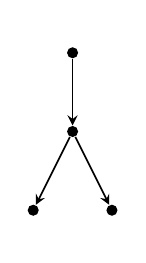
\begin{tikzpicture}[
		every label/.style={font=\scriptsize},
		state/.style={inner sep=0pt,fill,minimum size=4pt,circle,font=\scriptsize},
		arc/.style={->,>=stealth,semithick},
		probability/.style={-,densely dashed},
	]

\node at (1.5,1.2) {};
\node at (1.5,-1.2) {};
\node [state,label=] (s2) at (1.5,1.0) {};	

\node [inner sep=0pt,circle,fill,minimum size=4pt] (s2_1) at (1.5,0.0) {};

\node [inner sep=0pt,circle,fill,minimum size=4pt] (s2_2) at (1.0,-1.0) {};
\node [inner sep=0pt,circle,fill,minimum size=4pt] (s2_3) at (2.0,-1.0) {};

\draw [arc] (s2) to node [auto,pos=0.39,swap,font=\scriptsize] {} (s2_1);
\draw [arc] (s2_1) to node [swap,font=\scriptsize,anchor=base east] {} (s2_2);
\draw [arc] (s2_1) to node [font=\scriptsize,anchor=base west] {} (s2_3);


	
	\end{tikzpicture}
	\else
	\includegraphics{Pictures/counterex_pteallexists_trace_a}
	\fi
	
	&

	\ifwithtikz
\tikzsetnextfilename{counterex_pteallexists_trace_b}
	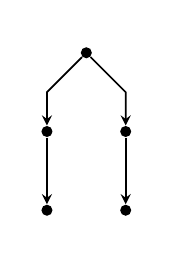
\begin{tikzpicture}[
		every label/.style={font=\scriptsize},
		state/.style={inner sep=0pt,fill,minimum size=4pt,circle,font=\scriptsize},
		arc/.style={->,>=stealth,semithick},
		probability/.style={-,densely dashed},
	]

\node at (1.5,1.2) {};
\node at (1.5,-1.2) {};
\node [state,label=] (s2) at (1.5,1.0) {};	

\node [inner sep=0pt,circle,fill,minimum size=4pt] (s2_1) at (1.0,0.0) {};
\node [inner sep=0pt,circle,fill,minimum size=4pt] (s2_4) at (2.0,0.0) {};

\node [inner sep=0pt,circle,fill,minimum size=4pt] (s2_5) at (1.0,-1.0) {};
\node [inner sep=0pt,circle,fill,minimum size=4pt] (s2_8) at (2.0,-1.0) {};

\draw [arc] (s2) to (1.0,0.5) to node [auto,pos=-0.2,swap,font=\scriptsize] {} (s2_1);
\draw [arc] (s2) to (2.0,0.5) to node [auto,pos=-0.2,font=\scriptsize] {} (s2_4);

\draw [arc] (s2_1) to node [swap,font=\scriptsize,anchor=base east] {}  (s2_5);
\draw [arc] (s2_4) to node [auto,font=\scriptsize,anchor=base west] {}  (s2_8);
	
	\end{tikzpicture}
	\else
	\includegraphics{Pictures/counterex_pteallexists_trace_b}
	\fi
	
	&

	\ifwithtikz
\tikzsetnextfilename{counterex_pteallexists_trace_c}
	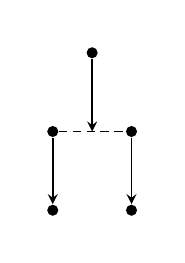
\begin{tikzpicture}[
		every label/.style={font=\scriptsize},
		state/.style={inner sep=0pt,fill,minimum size=4pt,circle,font=\scriptsize},
		arc/.style={->,>=stealth,semithick},
		probability/.style={-,densely dashed},
	]

\node at (1.5,1.2) {};
\node at (1.5,-1.2) {};
\node [state,label=] (s2) at (1.5,1.0) {};	

\node [inner sep=0pt,circle,fill,minimum size=4pt,label=] (s2_1) at (1.0,0.0) {};
\node [inner sep=0pt,circle,fill,minimum size=4pt,label=] (s2_4) at (2.0,0.0) {};

\node [inner sep=0pt,circle,fill,minimum size=4pt,label=left:] (s2_5) at (1.0,-1.0) {};
\node [inner sep=0pt,circle,fill,minimum size=4pt,label=right:] (s2_8) at (2.0,-1.0) {};

\draw [arc] (s2) to node [auto,pos=0.35,swap,font=\scriptsize] {} (1.5,0.0);

\draw [probability] (s2_1) -- (s2_4);

\draw [arc] (s2_1) to node [auto,swap,font=\scriptsize,anchor=base east] {}  (s2_5);
\draw [arc] (s2_4) to node [auto,font=\scriptsize,anchor=base west] {}  (s2_8);
	
	\end{tikzpicture}
	\else
	\includegraphics{Pictures/counterex_pteallexists_trace_c}
	\fi
	
	&

	\ifwithtikz
\tikzsetnextfilename{counterex_pteallexists_trace_d}
	\begin{tikzpicture}[
		every label/.style={font=\scriptsize},
		state/.style={inner sep=0pt,fill,minimum size=4pt,circle,font=\scriptsize},
		arc/.style={->,>=stealth,semithick},
		probability/.style={-,densely dashed},
	]

\node at (1.5,1.2) {};
\node at (1.5,-1.2) {};
\node [state,label={}] (s2) at (1.5,1.0) {};	

\node [inner sep=0pt,circle,fill,minimum size=4pt,label=] (s2_1) at (1.0,0.0) {};
\node [inner sep=0pt,circle,fill,minimum size=4pt,label=] (s2_4) at (2.0,0.0) {};

\node [inner sep=0pt,circle,fill,minimum size=4pt,label=left:] (s2_5) at (0.5,-1.0) {};
\node [inner sep=0pt,circle,fill,minimum size=4pt,label=right:] (s2_8) at (2.5,-1.0) {};

\draw [arc] (s2) to node [auto,pos=0.35,swap,font=\scriptsize] {} (1.5,0.0);

\draw [probability] (s2_1) -- (s2_4);

\draw [arc] (s2_1) to node [auto,swap,font=\scriptsize,anchor=base east] {}  (s2_5);
\draw [arc] (s2_4) to node [auto,font=\scriptsize,anchor=base west] {}  (s2_8);
	
	\end{tikzpicture}
	\else
	\includegraphics{Pictures/counterex_pteallexists_trace_d}
	\fi
	
	&

	\ifwithtikz
\tikzsetnextfilename{counterex_pteallexists_trace_e}
	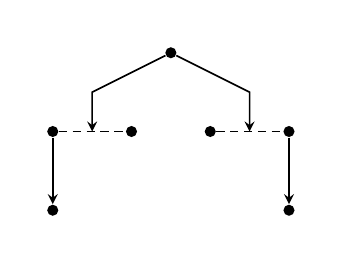
\begin{tikzpicture}[
		every label/.style={font=\scriptsize},
		state/.style={inner sep=0pt,fill,minimum size=4pt,circle,font=\scriptsize},
		arc/.style={->,>=stealth,semithick},
		probability/.style={-,densely dashed},
	]

\node at (1.5,1.2) {};
\node at (1.5,-1.2) {};
\node [state,label={}] (s2) at (2.5,1.0) {};	

\node [inner sep=0pt,circle,fill,minimum size=4pt,label=] (s2_1) at (1.0,0.0) {};
\node [inner sep=0pt,circle,fill,minimum size=4pt,label=] (s2_2) at (2.0,0.0) {};
\node [inner sep=0pt,circle,fill,minimum size=4pt,label=] (s2_3) at (3.0,0.0) {};
\node [inner sep=0pt,circle,fill,minimum size=4pt,label=] (s2_4) at (4.0,0.0) {};

\node [inner sep=0pt,circle,fill,minimum size=4pt,label=left:] (s2_5) at (1.0,-1.0) {};
\node [inner sep=0pt,circle,fill,minimum size=4pt,label=right:] (s2_8) at (4.0,-1.0) {};

\draw [arc] (s2) to (1.5,0.5) to node [auto,pos=-0.2,swap,font=\scriptsize] {} (1.5,0.0);
\draw [arc] (s2) to (3.5,0.5) to node [auto,pos=-0.2,font=\scriptsize] {} (3.5,0.0);

\draw [probability] (s2_1) -- (s2_2);
\draw [probability] (s2_3) -- (s2_4);

\draw [arc] (s2_1) to node [auto,swap,font=\scriptsize,anchor=base east] {}  (s2_5);
\draw [arc] (s2_4) to node [auto,font=\scriptsize,anchor=base west] {}  (s2_8);
	
	\end{tikzpicture} 
		\else
	\includegraphics{Pictures/counterex_pteallexists_trace_e}
	\fi
	\\
	
	\multicolumn{2}{c}{
	\emph{\small processes}
	}
	 & \emph{\small test} &
	\multicolumn{2}{c}{
	\emph{\small interaction systems}
	}

	\end{tabular}

	\end{center}
 \caption{NPLTS models identified by  and told apart by }
\label{fig:counterex_pteallexists_trace}

	\end{figure}

The inclusion of  in  is strict.
Indeed, if we consider again the two -equivalent NPLTS models in
Fig.~\ref{fig:counterex_ptesupinf_trace} and we apply the test in Fig.~\ref{fig:test_pteallexists}, it turns
out that . For the two interaction systems in
Fig.~\ref{fig:test_pteallexists}, we have that the maximal resolution of  starting with the
central -transition gives rise to a success probability equal to~0.25 that is not matched by any of the
two maximal resolutions of . These resolutions, which correspond to the maximal resolutions of
 starting with the two outermost -transitions, have success probability 0.5 and 0,
respectively.

	\begin{thm}\label{thm:pteallexists_incl_ptr}

Let  be an NPLTS and . Then:
\cws{12}{s_{1} \sbis{\textrm{{\rm PTe}-}\forall\exists} s_{2} \: \Longrightarrow \: s_{1} \sbis{\rm PTr}
s_{2}}

\proof
If , then in particular for every NPT  with initial state  having a single maximal computation that is
labeled with  and reaches success, it holds that:

		\begin{itemize}

\item For each  there exists  such that:
\cws{10}{\hspace*{-1.2cm} \ms{prob}(\calsc(z_{s_{1}, o})) \: = \: \ms{prob}(\calsc(z_{s_{2}, o}))}

\item For each  there exists  such that:
\cws{10}{\hspace*{-1.2cm} \ms{prob}(\calsc(z_{s_{2}, o})) \: = \: \ms{prob}(\calsc(z_{s_{1}, o}))}

		\end{itemize}

\noindent
Since  for all 
due to the structure of~ -- where  and  originates  in the interaction with  -- we immediately derive that for
all  it holds that:

		\begin{itemize}

\item For each  there exists  such that:
\cws{10}{\hspace*{-1.2cm} \ms{prob}(\calcc(z_{s_{1}}, \alpha)) \: = \: \ms{prob}(\calcc(z_{s_{2}}, \alpha))}

\item For each  there exists  such that:
\cws{10}{\hspace*{-1.2cm} \ms{prob}(\calcc(z_{s_{2}}, \alpha)) \: = \: \ms{prob}(\calcc(z_{s_{1}}, \alpha))}

		\end{itemize}

\noindent
This means that .	
\qed 

	\end{thm}

The inclusion of  in  is strict. For instance, if we
consider the two NPLTS models in Fig.~\ref{fig:counterex_pteallexists_trace}, it turns out that  while . In fact, the test in
Fig.~\ref{fig:counterex_pteallexists_trace} distinguishes~ from~ with respect to
 because -- looking at the two interaction systems also reported in the
figure -- the only maximal resolution of  has a success probability equal to 1 that is not
matched by any of the two maximal resolutions of , whose success probabilities are  and
, respectively.

Another desirable property of relations like  and
 that are defined over a general class of processes is that of being
backward compatible with analogous relations for restricted classes of processes. Specifically, we refer to
testing equivalences  for fully nondeterministic processes~\cite{DH84},  for fully probabilistic processes~\cite{CDSY99}, and  for reactive probabilistic
processes inspired by~\cite{KN98}.

	\begin{figure}[tp]

	\begin{center}

	\begin{tabular}{cc@{\hspace{0.5cm}}c@{\hspace{0.5cm}}cc}

	\ifwithtikz
\tikzsetnextfilename{counterex_tefnd_testing_a}	
	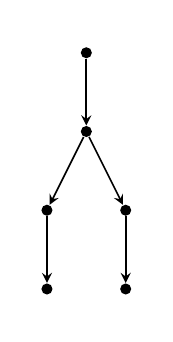
\begin{tikzpicture}[
		every label/.style={font=\scriptsize},
		state/.style={inner sep=0pt,fill,minimum size=4pt,circle,font=\scriptsize},
		arc/.style={->,>=stealth,semithick},
		probability/.style={-,densely dashed},
	]

\node at (1.5,1.2) {};
\node at (1.5,-2.2) {};
\node [state,label=] (s1) at (1.5,1.0) {};	

\node [inner sep=0pt,circle,fill,minimum size=4pt] (s1_1) at (1.5,0.0) {};

\node [inner sep=0pt,circle,fill,minimum size=4pt] (s1_2) at (1.0,-1.0) {};
\node [inner sep=0pt,circle,fill,minimum size=4pt] (s1_3) at (2.0,-1.0) {};

\node [inner sep=0pt,circle,fill,minimum size=4pt] (s1_4) at (1.0,-2.0) {};
\node [inner sep=0pt,circle,fill,minimum size=4pt] (s1_5) at (2.0,-2.0) {};


\draw [arc] (s1) to node [auto,pos=0.35,swap,font=\scriptsize] {} (s1_1);
\draw [arc] (s1_1) to node [font=\scriptsize,anchor=base east] {} (s1_2);
\draw [arc] (s1_1) to node [font=\scriptsize,anchor=base west] {} (s1_3);
\draw [arc] (s1_2) to node [font=\scriptsize,anchor=base east] {} (s1_4);
\draw [arc] (s1_3) to node [font=\scriptsize,anchor=base west] {} (s1_5);

	
	\end{tikzpicture}	
	\else
	\includegraphics{Pictures/counterex_tefnd_testing_a}
	\fi
	
	&

	\ifwithtikz
\tikzsetnextfilename{counterex_tefnd_testing_b}
	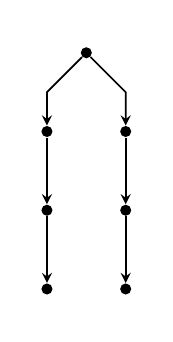
\begin{tikzpicture}[
		every label/.style={font=\scriptsize},
		state/.style={inner sep=0pt,fill,minimum size=4pt,circle,font=\scriptsize},
		arc/.style={->,>=stealth,semithick},
		probability/.style={-,densely dashed},
	]

\node at (1.5,1.2) {};
\node at (1.5,-2.2) {};
\node [state,label=] (s2) at (1.5,1.0) {};	

\node [inner sep=0pt,circle,fill,minimum size=4pt] (s2_1) at (1.0,0.0) {};
\node [inner sep=0pt,circle,fill,minimum size=4pt] (s2_2) at (2.0,0.0) {};

\node [inner sep=0pt,circle,fill,minimum size=4pt] (s2_3) at (1.0,-1.0) {};
\node [inner sep=0pt,circle,fill,minimum size=4pt] (s2_4) at (2.0,-1.0) {};

\node [inner sep=0pt,circle,fill,minimum size=4pt] (s2_5) at (1.0,-2.0) {};
\node [inner sep=0pt,circle,fill,minimum size=4pt] (s2_6) at (2.0,-2.0) {};


\draw [arc] (s2) to (1.0,0.5) to node [auto,pos=-0.2,swap,font=\scriptsize] {}  (s2_1);
\draw [arc] (s2) to (2.0,0.5) to node [auto,pos=-0.2,font=\scriptsize] {} (s2_2);

\draw [arc] (s2_1) to node [auto,swap,font=\scriptsize,anchor=base east] {}  (s2_3);
\draw [arc] (s2_2) to node [auto,font=\scriptsize,anchor=base west] {}  (s2_4);

\draw [arc] (s2_3) to node [auto,swap,font=\scriptsize,anchor=base east] {} (s2_5);
\draw [arc] (s2_4) to node [auto,font=\scriptsize,anchor=base west] {} (s2_6);
	
	\end{tikzpicture}	
	\else
	\includegraphics{Pictures/counterex_tefnd_testing_b}
	\fi
	
	&

	\ifwithtikz
\tikzsetnextfilename{counterex_tefnd_testing_c}
	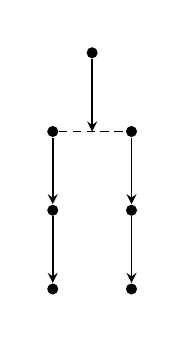
\begin{tikzpicture}[
		every label/.style={font=\scriptsize},
		state/.style={inner sep=0pt,fill,minimum size=4pt,circle,font=\scriptsize},
		arc/.style={->,>=stealth,semithick},
		probability/.style={-,densely dashed},
	]

\node at (1.5,1.2) {};
\node at (1.5,-2.2) {};
\node [state,label=] (s2) at (1.5,1.0) {};	

\node [inner sep=0pt,circle,fill,minimum size=4pt,label=] (s2_1) at (1.0,0.0) {};
\node [inner sep=0pt,circle,fill,minimum size=4pt,label=] (s2_2) at (2.0,0.0) {};

\node [inner sep=0pt,circle,fill,minimum size=4pt] (s2_3) at (1.0,-1.0) {};
\node [inner sep=0pt,circle,fill,minimum size=4pt] (s2_4) at (2.0,-1.0) {};

\node [inner sep=0pt,circle,fill,minimum size=4pt,label=left:] (s2_5) at (1.0,-2.0) {};
\node [inner sep=0pt,circle,fill,minimum size=4pt,label=right:] (s2_6) at (2.0,-2.0) {};

\draw [arc] (s2) to node [auto,pos=0.35,swap,font=\scriptsize] {} (1.5,0.0);

\draw [probability] (s2_1) -- (s2_2);

\draw [arc] (s2_1) to node [auto,swap,font=\scriptsize,anchor=base east] {}  (s2_3);
\draw [arc] (s2_2) to node [auto,font=\scriptsize,anchor=base west] {}  (s2_4);

\draw [arc] (s2_3) to node [auto,swap,font=\scriptsize,anchor=base east] {} (s2_5);
\draw [arc] (s2_4) to node [auto,font=\scriptsize,anchor=base west] {}(s2_6);
	
	\end{tikzpicture}
	\else
	\includegraphics{Pictures/counterex_tefnd_testing_c}
	\fi
	
	&

	\ifwithtikz
\tikzsetnextfilename{counterex_tefnd_testing_d}
	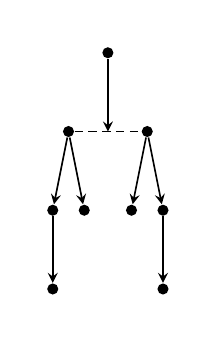
\begin{tikzpicture}[
		every label/.style={font=\scriptsize},
		state/.style={inner sep=0pt,fill,minimum size=4pt,circle,font=\scriptsize},
		arc/.style={->,>=stealth,semithick},
		probability/.style={-,densely dashed},
	]

\node at (1.5,1.2) {};
\node at (1.5,-2.2) {};
\node [state,label={}] (s2) at (1.5,1.0) {};	

\node [inner sep=0pt,circle,fill,minimum size=4pt,label=] (s2_1) at (1.0,0.0) {};
\node [inner sep=0pt,circle,fill,minimum size=4pt,label=] (s2_2) at (2.0,0.0) {};

\node [inner sep=0pt,circle,fill,minimum size=4pt] (s2_3) at (0.8,-1.0) {};
\node [inner sep=0pt,circle,fill,minimum size=4pt] (s2_4) at (1.2,-1.0) {};
\node [inner sep=0pt,circle,fill,minimum size=4pt] (s2_5) at (1.8,-1.0) {};
\node [inner sep=0pt,circle,fill,minimum size=4pt] (s2_6) at (2.2,-1.0) {};

\node [inner sep=0pt,circle,fill,minimum size=4pt,label=left:] (s2_7) at (0.8,-2.0) {};
\node [inner sep=0pt,circle,fill,minimum size=4pt,label=right:] (s2_8) at (2.2,-2.0) {};

\draw [arc] (s2) to node [auto,pos=0.35,swap,font=\scriptsize] {} (1.5,0.0);

\draw [probability] (s2_1) -- (s2_2);

\draw [arc] (s2_1) to node [auto,swap,font=\scriptsize,anchor=base east] {} (s2_3);
\draw [arc] (s2_1) to  node [auto,font=\scriptsize,anchor=base west] {} (s2_4);
\draw [arc] (s2_2) to node [auto,swap,font=\scriptsize,anchor=base east] {} (s2_5);
\draw [arc] (s2_2) to node [auto,font=\scriptsize,anchor=base west] {} (s2_6);

\draw [arc] (s2_3) to node [auto,swap,font=\scriptsize,anchor=base east] {} (s2_7);
\draw [arc] (s2_6) to node [auto,,font=\scriptsize,anchor=base west] {} (s2_8);
	
	\end{tikzpicture}
	\else
	\includegraphics{Pictures/counterex_tefnd_testing_d}
	\fi
	
	&

	\ifwithtikz
\tikzsetnextfilename{counterex_tefnd_testing_e}
	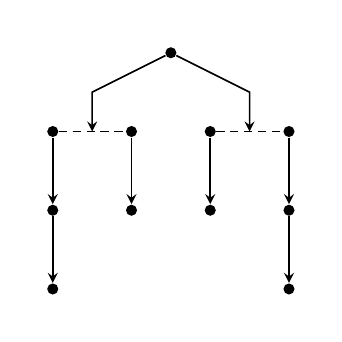
\begin{tikzpicture}[
		every label/.style={font=\scriptsize},
		state/.style={inner sep=0pt,fill,minimum size=4pt,circle,font=\scriptsize},
		arc/.style={->,>=stealth,semithick},
		probability/.style={-,densely dashed},
	]

\node at (2.5,1.2) {};
\node at (2.5,-2.2) {};
\node [state,label={}] (s2) at (2.5,1.0) {};	

\node [inner sep=0pt,circle,fill,minimum size=4pt,label=] (s2_1) at (1.0,0.0) {};
\node [inner sep=0pt,circle,fill,minimum size=4pt,label=] (s2_2) at (2.0,0.0) {};
\node [inner sep=0pt,circle,fill,minimum size=4pt,label=] (s2_3) at (3.0,0.0) {};
\node [inner sep=0pt,circle,fill,minimum size=4pt,label=] (s2_4) at (4.0,0.0) {};

\node [inner sep=0pt,circle,fill,minimum size=4pt] (s2_5) at (1.0,-1.0) {};
\node [inner sep=0pt,circle,fill,minimum size=4pt] (s2_6) at (2.0,-1.0) {};
\node [inner sep=0pt,circle,fill,minimum size=4pt] (s2_7) at (3.0,-1.0) {};
\node [inner sep=0pt,circle,fill,minimum size=4pt] (s2_8) at (4.0,-1.0) {};

\node [inner sep=0pt,circle,fill,minimum size=4pt,label=left:] (s2_9) at (1.0,-2.0) {};
\node [inner sep=0pt,circle,fill,minimum size=4pt,label=right:] (s2_10) at (4.0,-2.0) {};

\draw [arc] (s2) to (1.5,0.5) to node [auto,pos=-0.2,swap,font=\scriptsize] {} (1.5,0.0);
\draw [arc] (s2) to (3.5,0.5) to node [auto,pos=-0.2,font=\scriptsize] {} (3.5,0.0);

\draw [probability] (s2_1) -- (s2_2);
\draw [probability] (s2_3) -- (s2_4);

\draw [arc] (s2_1) to node [auto,swap,font=\scriptsize,anchor=base east] {}  (s2_5);
\draw [arc] (s2_2) to node [auto,font=\scriptsize,anchor=base west] {}  (s2_6);
\draw [arc] (s2_3) to node [auto,swap,font=\scriptsize,anchor=base east] {}  (s2_7);
\draw [arc] (s2_4) to node [auto,font=\scriptsize,anchor=base west] {}  (s2_8);

\draw [arc] (s2_5) to node [auto,swap,font=\scriptsize,anchor=base east] {} (s2_9);
\draw [arc] (s2_8) to node [auto,swap,font=\scriptsize,anchor=base west] {} (s2_10);
	
	
	\end{tikzpicture} 
		\else
	\includegraphics{Pictures/counterex_tefnd_testing_e}
	\fi
	\\
	
		\multicolumn{2}{c}{
	\emph{\small processes}
	}
 & \emph{\small test} &
	\multicolumn{2}{c}{
	\emph{\small interaction systems}	
	}

	\end{tabular}
	\end{center}
 \caption{NPLTS models equated by  and distinguished by
/}
\label{fig:counterex_tefnd_testing}

	\end{figure}

	\begin{figure}

	\begin{center}
	
		\begin{tabular}{cccccc}

	\ifwithtikz
\tikzsetnextfilename{counterex_tefnd_testing_max_res_a}
	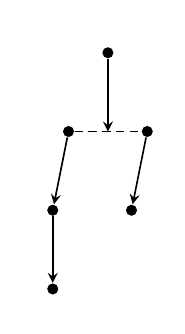
\begin{tikzpicture}[
		every label/.style={font=\scriptsize},
		state/.style={inner sep=0pt,fill,minimum size=4pt,circle,font=\scriptsize},
		arc/.style={->,>=stealth,semithick},
		probability/.style={-,densely dashed},
	]

\node at (1.5,1.1) {};
\node at (1.5,-2.1) {};
\node [state,label={}] (s2) at (1.5,1.0) {};	

\node [inner sep=0pt,circle,fill,minimum size=4pt,label=] (s2_1) at (1.0,0.0) {};
\node [inner sep=0pt,circle,fill,minimum size=4pt,label=] (s2_2) at (2.0,0.0) {};

\node [inner sep=0pt,circle,fill,minimum size=4pt] (s2_3) at (0.8,-1.0) {};
\node [inner sep=0pt,circle,fill,minimum size=4pt] (s2_5) at (1.8,-1.0) {};


\node [inner sep=0pt,circle,fill,minimum size=4pt,label=left:] (s2_7) at (0.8,-2.0) {};


\draw [arc] (s2) to node [auto,pos=0.35,swap,font=\scriptsize] {} (1.5,0.0);

\draw [probability] (s2_1) -- (s2_2);

\draw [arc] (s2_1) to node [auto,swap,font=\scriptsize,anchor=base east] {}  (s2_3);
\draw [arc] (s2_2) to node [auto,font=\scriptsize,anchor=base east] {}  (s2_5);


\draw [arc] (s2_3) to node [auto,swap,font=\scriptsize,anchor=base east] {}  (s2_7);


	\end{tikzpicture}
	\else
	\includegraphics{Pictures/counterex_tefnd_testing_max_res_a}
	\fi
	
	&

	\ifwithtikz
\tikzsetnextfilename{counterex_tefnd_testing_max_res_b}
	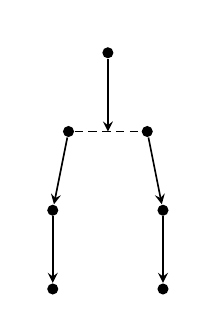
\begin{tikzpicture}[
		every label/.style={font=\scriptsize},
		state/.style={inner sep=0pt,fill,minimum size=4pt,circle,font=\scriptsize},
		arc/.style={->,>=stealth,semithick},
		probability/.style={-,densely dashed},
	]

\node at (1.5,1.1) {};
\node at (1.5,-2.1) {};
\node [state,label={}] (s2) at (1.5,1.0) {};	

\node [inner sep=0pt,circle,fill,minimum size=4pt,label=] (s2_1) at (1.0,0.0) {};
\node [inner sep=0pt,circle,fill,minimum size=4pt,label=] (s2_2) at (2.0,0.0) {};

\node [inner sep=0pt,circle,fill,minimum size=4pt] (s2_3) at (0.8,-1.0) {};
\node [inner sep=0pt,circle,fill,minimum size=4pt] (s2_6) at (2.2,-1.0) {};

\node [inner sep=0pt,circle,fill,minimum size=4pt,label=left:] (s2_7) at (0.8,-2.0) {};
\node [inner sep=0pt,circle,fill,minimum size=4pt,label=right:] (s2_8) at (2.2,-2.0) {};

\draw [arc] (s2) to node [auto,pos=0.35,swap,font=\scriptsize] {} (1.5,0.0);

\draw [probability] (s2_1) -- (s2_2);

\draw [arc] (s2_1) to node [auto,,swap,font=\scriptsize,anchor=base east] {}  (s2_3);
\draw [arc] (s2_2) to node [auto,font=\scriptsize,anchor=base west] {}  (s2_6);

\draw [arc] (s2_3) to node [auto,swap,font=\scriptsize,anchor=base east] {}  (s2_7);
\draw [arc] (s2_6) to node [auto,font=\scriptsize,anchor=base west] {}  (s2_8);
	
	\end{tikzpicture}
	\else
	\includegraphics{Pictures/counterex_tefnd_testing_max_res_b}
	\fi
	
	&

	\ifwithtikz
\tikzsetnextfilename{counterex_tefnd_testing_max_res_c}
	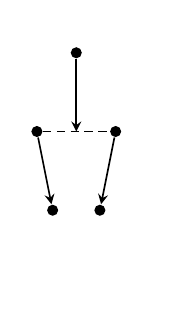
\begin{tikzpicture}[
		every label/.style={font=\scriptsize},
		state/.style={inner sep=0pt,fill,minimum size=4pt,circle,font=\scriptsize},
		arc/.style={->,>=stealth,semithick},
		probability/.style={-,densely dashed},
	]

\node at (1.5,1.1) {};
\node at (1.5,-2.1) {};
\node [state,label={}] (s2) at (1.5,1.0) {};	

\node [inner sep=0pt,circle,fill,minimum size=4pt,label=] (s2_1) at (1.0,0.0) {};
\node [inner sep=0pt,circle,fill,minimum size=4pt,label=] (s2_2) at (2.0,0.0) {};

\node [inner sep=0pt,circle,fill,minimum size=4pt] (s2_4) at (1.2,-1.0) {};
\node [inner sep=0pt,circle,fill,minimum size=4pt] (s2_5) at (1.8,-1.0) {};




\draw [arc] (s2) to node [auto,pos=0.35,swap,font=\scriptsize] {} (1.5,0.0);

\draw [probability] (s2_1) -- (s2_2);

\draw [arc] (s2_1) to node [auto,font=\scriptsize,anchor=base west] {}  (s2_4);
\draw [arc] (s2_2) to node [auto,swap,font=\scriptsize,anchor=base east] {}  (s2_5);


\node at (2.2,-2.0) {};
	
	\end{tikzpicture}
	\else
	\includegraphics{Pictures/counterex_tefnd_testing_max_res_c}
	\fi
	
	&

	\ifwithtikz
\tikzsetnextfilename{counterex_tefnd_testing_max_res_d}
	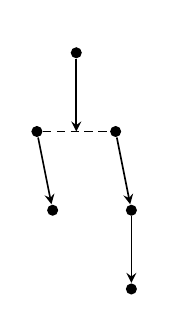
\begin{tikzpicture}[
		every label/.style={font=\scriptsize},
		state/.style={inner sep=0pt,fill,minimum size=4pt,circle,font=\scriptsize},
		arc/.style={->,>=stealth,semithick},
		probability/.style={-,densely dashed},
	]

\node at (1.5,1.1) {};
\node at (1.5,-2.1) {};
\node [state,label={}] (s2) at (1.5,1.0) {};	

\node [inner sep=0pt,circle,fill,minimum size=4pt,label=] (s2_1) at (1.0,0.0) {};
\node [inner sep=0pt,circle,fill,minimum size=4pt,label=] (s2_2) at (2.0,0.0) {};

\node [inner sep=0pt,circle,fill,minimum size=4pt] (s2_4) at (1.2,-1.0) {};
\node [inner sep=0pt,circle,fill,minimum size=4pt] (s2_6) at (2.2,-1.0) {};

\node [inner sep=0pt,circle,fill,minimum size=4pt,label=right:] (s2_8) at (2.2,-2.0) {};

\draw [arc] (s2) to node [auto,pos=0.35,swap,font=\scriptsize] {} (1.5,0.0);

\draw [probability] (s2_1) -- (s2_2);

\draw [arc] (s2_1) to node [auto,font=\scriptsize,anchor=base west] {}  (s2_4);
\draw [arc] (s2_2) to node [auto,font=\scriptsize,anchor=base west] {}  (s2_6);

\draw [arc] (s2_6) to node [auto,font=\scriptsize,anchor=base west] {}  (s2_8);
	
	\end{tikzpicture}
	\else
	\includegraphics{Pictures/counterex_tefnd_testing_max_res_d}
	\fi
	
	&

	\ifwithtikz
\tikzsetnextfilename{counterex_tefnd_testing_max_res_e}
	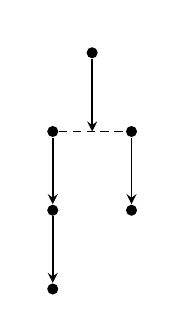
\begin{tikzpicture}[
		every label/.style={font=\scriptsize},
		state/.style={inner sep=0pt,fill,minimum size=4pt,circle,font=\scriptsize},
		arc/.style={->,>=stealth,semithick},
		probability/.style={-,densely dashed},
	]

\node at (1.5,1.1) {};
\node at (1.5,-2.1) {};
\node [state,label={}] (s2) at (1.5,1.0) {};	

\node [inner sep=0pt,circle,fill,minimum size=4pt,label=] (s2_1) at (1.0,0.0) {};
\node [inner sep=0pt,circle,fill,minimum size=4pt,label=] (s2_2) at (2.0,0.0) {};

\node [inner sep=0pt,circle,fill,minimum size=4pt] (s2_5) at (1.0,-1.0) {};
\node [inner sep=0pt,circle,fill,minimum size=4pt] (s2_6) at (2.0,-1.0) {};

\node [inner sep=0pt,circle,fill,minimum size=4pt,label=left:] (s2_9) at (1.0,-2.0) {};

\draw [arc] (s2) to node [auto,pos=0.35,swap,font=\scriptsize] {} (1.5,0.0);

\draw [probability] (s2_1) -- (s2_2);

\draw [arc] (s2_1) to node [auto,swap,font=\scriptsize,anchor=base east] {}  (s2_5);
\draw [arc] (s2_2) to node [auto,font=\scriptsize,anchor=base west] {}  (s2_6);

\draw [arc] (s2_5) to node [auto,swap,font=\scriptsize,anchor=base east] {}  (s2_9);
	
	\end{tikzpicture}
	\else
	\includegraphics{Pictures/counterex_tefnd_testing_max_res_e}
	\fi
	
	&

	\ifwithtikz
\tikzsetnextfilename{counterex_tefnd_testing_max_res_f}
	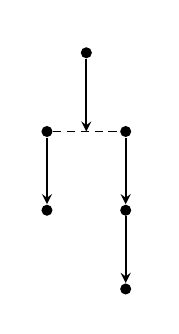
\begin{tikzpicture}[
		every label/.style={font=\scriptsize},
		state/.style={inner sep=0pt,fill,minimum size=4pt,circle,font=\scriptsize},
		arc/.style={->,>=stealth,semithick},
		probability/.style={-,densely dashed},
	]

\node at (3.5,1.1) {};
\node at (3.5,-2.1) {};
\node [state,label={}] (s2) at (3.5,1.0) {};	

\node [inner sep=0pt,circle,fill,minimum size=4pt,label=] (s2_3) at (3.0,0.0) {};
\node [inner sep=0pt,circle,fill,minimum size=4pt,label=] (s2_4) at (4.0,0.0) {};

\node [inner sep=0pt,circle,fill,minimum size=4pt] (s2_7) at (3.0,-1.0) {};
\node [inner sep=0pt,circle,fill,minimum size=4pt] (s2_8) at (4.0,-1.0) {};

\node [inner sep=0pt,circle,fill,minimum size=4pt,label=right:] (s2_10) at (4.0,-2.0) {};

\draw [arc] (s2) to node [auto,pos=0.35,swap,font=\scriptsize] {} (3.5,0.0);

\draw [probability] (s2_3) -- (s2_4);

\draw [arc] (s2_3) to node [auto,swap,font=\scriptsize,anchor=base east] {}  (s2_7);
\draw [arc] (s2_4) to node [auto,font=\scriptsize,anchor=base west] {}  (s2_8);

\draw [arc] (s2_8) to node [auto,font=\scriptsize,anchor=base west] {}  (s2_10);
	
	\end{tikzpicture}
	\else
	\includegraphics{Pictures/counterex_tefnd_testing_max_res_f}
	\fi
	
	\end{tabular}
	\end{center}
 \caption{Maximal resolutions of the two interaction systems in Fig.~\ref{fig:counterex_tefnd_testing}.}
\label{fig:counterex_tefnd_testing_max_res}

	\end{figure}

As we shall see by means of two counterexamples, backward compatibility is only \emph{partial} as it depends
on the set of tests that are used. Intuitively,  and
 become sensitive to the moment of occurrence of internal choices when
comparing fully nondeterministic processes (resp.\ fully/reactive probabilistic processes) on the basis of
tests admitting probabilities (resp.\ internal nondeterminism). In such cases, the capability of making
copies of intermediate states of the processes under test arises, a fact that in general increases the
distinguishing power of testing equivalence, as pointed out in~\cite{Abr87}. In a probabilistic setting,
this may lead to questionable estimations of success probabilities (see~\cite{GA12} and the references
therein). Indeed, taking advantage of the increased discriminating power, in~\cite{DGHM08} it was shown that
the may-part of  coincides with a simulation equivalence akin to the one
in~\cite{LSV03} and the must-part coincides with a novel failure simulation equivalence. Moreover,
in~\cite{Seg96} it was shown that the may-part coincides with the coarsest congruence contained in the
probabilistic trace-distribution equivalence of~\cite{Seg95b} and the must-part coincides with the coarsest
congruence contained in a probabilistic failure-distribution equivalence.

	\begin{figure}[tp]

	\begin{center}

	\begin{tabular}{cc@{\hspace{0.5cm}}c@{\hspace{0.5cm}}cc}

	\ifwithtikz
	\tikzsetnextfilename{counterex_tepr_testing_a}	
	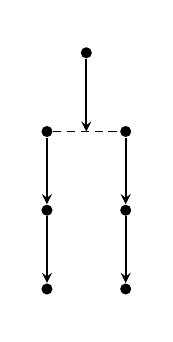
\begin{tikzpicture}[
		every label/.style={font=\scriptsize},
		state/.style={inner sep=0pt,fill,minimum size=4pt,circle,font=\scriptsize},
		arc/.style={->,>=stealth,semithick},
		probability/.style={-,densely dashed},
	]

\node at (1.5,1.2) {};
\node at (1.5,-2.2) {};
\node [state,label=] (s1) at (1.5,1.0) {};	

\node [inner sep=0pt,circle,fill,minimum size=4pt,label=] (s1_1a) at (1.0,0.0) {};
\node [inner sep=0pt,circle,fill,minimum size=4pt,label=] (s1_1b) at (2.0,0.0) {};

\node [inner sep=0pt,circle,fill,minimum size=4pt] (s1_2) at (1.0,-1.0) {};
\node [inner sep=0pt,circle,fill,minimum size=4pt] (s1_3) at (2.0,-1.0) {};

\node [inner sep=0pt,circle,fill,minimum size=4pt] (s1_4) at (1.0,-2.0) {};
\node [inner sep=0pt,circle,fill,minimum size=4pt] (s1_5) at (2.0,-2.0) {};

\draw [probability] (s1_1a) -- (s1_1b);

\draw [arc] (s1) to node [auto,swap,pos=0.35,font=\scriptsize] {} (1.5,0.0);
\draw [arc] (s1_1a) to node [auto,swap,font=\scriptsize,anchor=base east] {} (s1_2);
\draw [arc] (s1_1b) to node [auto,font=\scriptsize,anchor=base west] {} (s1_3);
\draw [arc] (s1_2) to node [auto,swap,font=\scriptsize,anchor=base east] {} (s1_4);
\draw [arc] (s1_3) to node [auto,font=\scriptsize,anchor=base west] {} (s1_5);

	
	\end{tikzpicture}	
	\else
	\includegraphics{Pictures/counterex_tepr_testing_a}
	\fi
	
	&

	\ifwithtikz
	\tikzsetnextfilename{counterex_tepr_testing_b}
	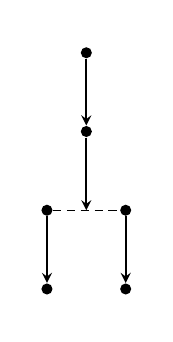
\begin{tikzpicture}[
		every label/.style={font=\scriptsize},
		state/.style={inner sep=0pt,fill,minimum size=4pt,circle,font=\scriptsize},
		arc/.style={->,>=stealth,semithick},
		probability/.style={-,densely dashed},
	]

\node at (1.5,1.2) {};
\node at (1.5,-2.2) {};
\node [state,label=] (s2) at (1.5,1.0) {};	

\node [inner sep=0pt,circle,fill,minimum size=4pt] (s2_1) at (1.5,0.0) {};

\node [inner sep=0pt,circle,fill,minimum size=4pt,label=] (s2_2) at (1.0,-1.0) {};
\node [inner sep=0pt,circle,fill,minimum size=4pt,label=] (s2_3) at (2.0,-1.0) {};

\node [inner sep=0pt,circle,fill,minimum size=4pt] (s2_4) at (1.0,-2.0) {};
\node [inner sep=0pt,circle,fill,minimum size=4pt] (s2_5) at (2.0,-2.0) {};

\draw [probability] (s2_2) -- (s2_3);

\draw [arc] (s2) to node [auto,swap,pos=0.38,font=\scriptsize] {}  (s2_1);

\draw [arc] (s2_1) to node [auto,swap,font=\scriptsize,pos=0.45,anchor=base east] {}  (1.5,-1);

\draw [arc] (s2_2) to node [auto,swap,font=\scriptsize,anchor=base east] {}  (s2_4);
\draw [arc] (s2_3) to node [auto,font=\scriptsize,anchor=base west] {}  (s2_5);
	
	\end{tikzpicture}	
	\else
	\includegraphics{Pictures/counterex_tepr_testing_b}
	\fi
	
	&

	\ifwithtikz
	\tikzsetnextfilename{counterex_tepr_testing_c}
	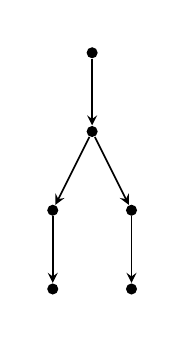
\begin{tikzpicture}[
		every label/.style={font=\scriptsize},
		state/.style={inner sep=0pt,fill,minimum size=4pt,circle,font=\scriptsize},
		arc/.style={->,>=stealth,semithick},
		probability/.style={-,densely dashed},
	]

\node at (1.5,1.2) {};
\node at (1.5,-2.2) {};
\node [state,label=] (s2) at (1.5,1.0) {};	

\node [inner sep=0pt,circle,fill,minimum size=4pt] (s2_1) at (1.5,0.0) {};

\node [inner sep=0pt,circle,fill,minimum size=4pt] (s2_2) at (1.0,-1.0) {};
\node [inner sep=0pt,circle,fill,minimum size=4pt] (s2_3) at (2.0,-1.0) {};

\node [inner sep=0pt,circle,fill,minimum size=4pt,label=left:] (s2_4) at (1.0,-2.0) {};
\node [inner sep=0pt,circle,fill,minimum size=4pt,label=right:] (s2_5) at (2.0,-2.0) {};

\draw [arc] (s2) to node [auto,swap,pos=0.35,font=\scriptsize] {} (s2_1);

\draw [arc] (s2_1) to node [auto,swap,font=\scriptsize,anchor=base east] {}  (s2_2);
\draw [arc] (s2_1) to node [auto,font=\scriptsize,anchor=base west] {}  (s2_3);

\draw [arc] (s2_2) to node [auto,swap,font=\scriptsize,anchor=base east] {}  (s2_4);
\draw [arc] (s2_3) to node [auto,font=\scriptsize,anchor=base west] {}  (s2_5);
	
	\end{tikzpicture}
	\else
	\includegraphics{Pictures/counterex_tepr_testing_c}
	\fi
	
	&

	\ifwithtikz
	\tikzsetnextfilename{counterex_tepr_testing_d}
	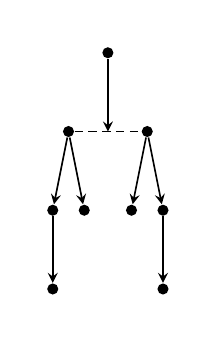
\begin{tikzpicture}[
		every label/.style={font=\scriptsize},
		state/.style={inner sep=0pt,fill,minimum size=4pt,circle,font=\scriptsize},
		arc/.style={->,>=stealth,semithick},
		probability/.style={-,densely dashed},
	]

\node at (1.5,1.2) {};
\node at (1.5,-2.2) {};
\node [state,label={}] (s2) at (1.5,1.0) {};	

\node [inner sep=0pt,circle,fill,minimum size=4pt,label=] (s2_1) at (1.0,0.0) {};
\node [inner sep=0pt,circle,fill,minimum size=4pt,label=] (s2_2) at (2.0,0.0) {};

\node [inner sep=0pt,circle,fill,minimum size=4pt] (s2_3) at (0.8,-1.0) {};
\node [inner sep=0pt,circle,fill,minimum size=4pt] (s2_4) at (1.2,-1.0) {};
\node [inner sep=0pt,circle,fill,minimum size=4pt] (s2_5) at (1.8,-1.0) {};
\node [inner sep=0pt,circle,fill,minimum size=4pt] (s2_6) at (2.2,-1.0) {};

\node [inner sep=0pt,circle,fill,minimum size=4pt,label=left:] (s2_7) at (0.8,-2.0) {};
\node [inner sep=0pt,circle,fill,minimum size=4pt,label=right:] (s2_8) at (2.2,-2.0) {};

\draw [arc] (s2) to node [auto,swap,pos=0.35,font=\scriptsize] {} (1.5,0.0);

\draw [probability] (s2_1) -- (s2_2);

\draw [arc] (s2_1) to node [auto,swap,font=\scriptsize,anchor=base east] {}  (s2_3);
\draw [arc] (s2_1) to node [auto,font=\scriptsize,anchor=base west] {}  (s2_4);
\draw [arc] (s2_2) to node [auto,swap,font=\scriptsize,anchor=base east] {}  (s2_5);
\draw [arc] (s2_2) to node [auto,font=\scriptsize,anchor=base west] {}  (s2_6);

\draw [arc] (s2_3) to node [auto,swap,font=\scriptsize,anchor=base east] {}  (s2_7);
\draw [arc] (s2_6) to node [auto,font=\scriptsize,anchor=base west] {}  (s2_8);
	
	\end{tikzpicture}
	\else
	\includegraphics{Pictures/counterex_tepr_testing_d}
	\fi
	
	&

	\ifwithtikz
	\tikzsetnextfilename{counterex_tepr_testing_e}
	\begin{tikzpicture}[
		every label/.style={font=\scriptsize},
		state/.style={inner sep=0pt,fill,minimum size=4pt,circle,font=\scriptsize},
		arc/.style={->,>=stealth,semithick},
		probability/.style={-,densely dashed},
	]

\node at (1.5,1.2) {};
\node at (1.5,-2.2) {};
\node [state,label={}] (s2) at (2.5,1.0) {};	

\node [inner sep=0pt,circle,fill,minimum size=4pt] (s2_1) at (2.5,0.0) {};

\node [inner sep=0pt,circle,fill,minimum size=4pt,label=] (s2_2) at (1.0,-1.0) {};
\node [inner sep=0pt,circle,fill,minimum size=4pt,label=] (s2_3) at (2.0,-1.0) {};
\node [inner sep=0pt,circle,fill,minimum size=4pt,label=] (s2_4) at (3.0,-1.0) {};
\node [inner sep=0pt,circle,fill,minimum size=4pt,label=] (s2_5) at (4.0,-1.0) {};

\node [inner sep=0pt,circle,fill,minimum size=4pt,label=left:] (s2_6) at (1.0,-2.0) {};
\node [inner sep=0pt,circle,fill,minimum size=4pt,label=right:] (s2_7) at (4.0,-2.0) {};

\draw [arc] (s2) to node [auto,swap,pos=0.35,font=\scriptsize] {} (s2_1);

\draw [probability] (s2_2) -- (s2_3);
\draw [probability] (s2_4) -- (s2_5);

\draw [arc] (s2_1) to (1.5,-0.5) to node [auto,pos=-0.2,swap,font=\scriptsize] {}  (1.5,-1);
\draw [arc] (s2_1) to (3.5,-0.5) to node [auto,pos=-0.2,font=\scriptsize] {} (3.5,-1);


\draw [arc] (s2_2) to node [auto,swap,font=\scriptsize,anchor=base east] {}  (s2_6);
\draw [arc] (s2_5) to node [auto,font=\scriptsize,anchor=base west] {}  (s2_7);
	
	\end{tikzpicture} 
		\else
	\includegraphics{Pictures/counterex_tepr_testing_e}
	\fi
	\\
	
		\multicolumn{2}{c}{
	\emph{processes}
	}
 & \emph{test} &
	\multicolumn{2}{c}{
	\emph{interaction systems}	
	}

	\end{tabular}
	\end{center}
 \caption{NPLTS models equated by / and distinguished by
/}
\label{fig:counterex_tepr_testing}

	\end{figure}

	\begin{figure}

	\begin{center}
	
		\begin{tabular}{cccccc}

	\ifwithtikz
\tikzsetnextfilename{counterex_tepr_testing_max_res_a}
	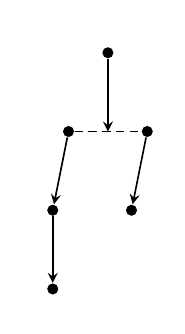
\begin{tikzpicture}[
		every label/.style={font=\scriptsize},
		state/.style={inner sep=0pt,fill,minimum size=4pt,circle,font=\scriptsize},
		arc/.style={->,>=stealth,semithick},
		probability/.style={-,densely dashed},
	]

\node at (1.5,1.1) {};
\node at (1.5,-2.1) {};
\node [state,label={}] (s2) at (1.5,1.0) {};	

\node [inner sep=0pt,circle,fill,minimum size=4pt,label=] (s2_1) at (1.0,0.0) {};
\node [inner sep=0pt,circle,fill,minimum size=4pt,label=] (s2_2) at (2.0,0.0) {};

\node [inner sep=0pt,circle,fill,minimum size=4pt] (s2_3) at (0.8,-1.0) {};
\node [inner sep=0pt,circle,fill,minimum size=4pt] (s2_5) at (1.8,-1.0) {};


\node [inner sep=0pt,circle,fill,minimum size=4pt,label=left:] (s2_7) at (0.8,-2.0) {};


\draw [arc] (s2) to node [auto,pos=0.35,swap,font=\scriptsize] {} (1.5,0.0);

\draw [probability] (s2_1) -- (s2_2);

\draw [arc] (s2_1) to node [auto,swap,font=\scriptsize,anchor=base east] {}  (s2_3);
\draw [arc] (s2_2) to node [auto,font=\scriptsize,anchor=base east] {}  (s2_5);


\draw [arc] (s2_3) to node [auto,swap,font=\scriptsize,anchor=base east] {}  (s2_7);


	\end{tikzpicture}
	\else
	\includegraphics{Pictures/counterex_tepr_testing_max_res_a}
	\fi
	
	&

	\ifwithtikz
\tikzsetnextfilename{counterex_tepr_testing_max_res_b}
	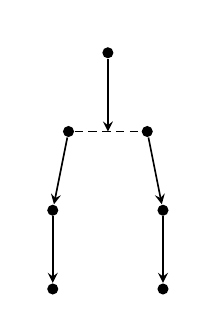
\begin{tikzpicture}[
		every label/.style={font=\scriptsize},
		state/.style={inner sep=0pt,fill,minimum size=4pt,circle,font=\scriptsize},
		arc/.style={->,>=stealth,semithick},
		probability/.style={-,densely dashed},
	]

\node at (1.5,1.1) {};
\node at (1.5,-2.1) {};
\node [state,label={}] (s2) at (1.5,1.0) {};	

\node [inner sep=0pt,circle,fill,minimum size=4pt,label=] (s2_1) at (1.0,0.0) {};
\node [inner sep=0pt,circle,fill,minimum size=4pt,label=] (s2_2) at (2.0,0.0) {};

\node [inner sep=0pt,circle,fill,minimum size=4pt] (s2_3) at (0.8,-1.0) {};
\node [inner sep=0pt,circle,fill,minimum size=4pt] (s2_6) at (2.2,-1.0) {};

\node [inner sep=0pt,circle,fill,minimum size=4pt,label=left:] (s2_7) at (0.8,-2.0) {};
\node [inner sep=0pt,circle,fill,minimum size=4pt,label=right:] (s2_8) at (2.2,-2.0) {};

\draw [arc] (s2) to node [auto,pos=0.35,swap,font=\scriptsize] {} (1.5,0.0);

\draw [probability] (s2_1) -- (s2_2);

\draw [arc] (s2_1) to node [auto,,swap,font=\scriptsize,anchor=base east] {}  (s2_3);
\draw [arc] (s2_2) to node [auto,font=\scriptsize,anchor=base west] {}  (s2_6);

\draw [arc] (s2_3) to node [auto,swap,font=\scriptsize,anchor=base east] {}  (s2_7);
\draw [arc] (s2_6) to node [auto,font=\scriptsize,anchor=base west] {}  (s2_8);
	
	\end{tikzpicture}
	\else
	\includegraphics{Pictures/counterex_tepr_testing_max_res_b}
	\fi
	
	&

	\ifwithtikz
\tikzsetnextfilename{counterex_tepr_testing_max_res_c}
	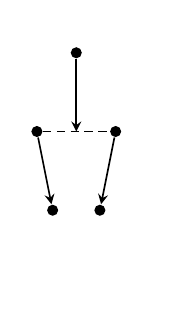
\begin{tikzpicture}[
		every label/.style={font=\scriptsize},
		state/.style={inner sep=0pt,fill,minimum size=4pt,circle,font=\scriptsize},
		arc/.style={->,>=stealth,semithick},
		probability/.style={-,densely dashed},
	]

\node at (1.5,1.1) {};
\node at (1.5,-2.1) {};
\node [state,label={}] (s2) at (1.5,1.0) {};	

\node [inner sep=0pt,circle,fill,minimum size=4pt,label=] (s2_1) at (1.0,0.0) {};
\node [inner sep=0pt,circle,fill,minimum size=4pt,label=] (s2_2) at (2.0,0.0) {};

\node [inner sep=0pt,circle,fill,minimum size=4pt] (s2_4) at (1.2,-1.0) {};
\node [inner sep=0pt,circle,fill,minimum size=4pt] (s2_5) at (1.8,-1.0) {};




\draw [arc] (s2) to node [auto,pos=0.35,swap,font=\scriptsize] {} (1.5,0.0);

\draw [probability] (s2_1) -- (s2_2);

\draw [arc] (s2_1) to node [auto,font=\scriptsize,anchor=base west] {}  (s2_4);
\draw [arc] (s2_2) to node [auto,swap,font=\scriptsize,anchor=base east] {}  (s2_5);


\node at (2.2,-2.0) {};
	
	\end{tikzpicture}
	\else
	\includegraphics{Pictures/counterex_tepr_testing_max_res_c}
	\fi
	
	&

	\ifwithtikz
\tikzsetnextfilename{counterex_tepr_testing_max_res_d}
	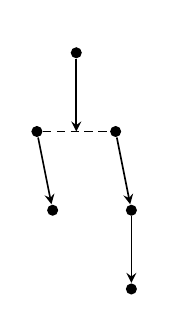
\begin{tikzpicture}[
		every label/.style={font=\scriptsize},
		state/.style={inner sep=0pt,fill,minimum size=4pt,circle,font=\scriptsize},
		arc/.style={->,>=stealth,semithick},
		probability/.style={-,densely dashed},
	]

\node at (1.5,1.1) {};
\node at (1.5,-2.1) {};
\node [state,label={}] (s2) at (1.5,1.0) {};	

\node [inner sep=0pt,circle,fill,minimum size=4pt,label=] (s2_1) at (1.0,0.0) {};
\node [inner sep=0pt,circle,fill,minimum size=4pt,label=] (s2_2) at (2.0,0.0) {};

\node [inner sep=0pt,circle,fill,minimum size=4pt] (s2_4) at (1.2,-1.0) {};
\node [inner sep=0pt,circle,fill,minimum size=4pt] (s2_6) at (2.2,-1.0) {};

\node [inner sep=0pt,circle,fill,minimum size=4pt,label=right:] (s2_8) at (2.2,-2.0) {};

\draw [arc] (s2) to node [auto,pos=0.35,swap,font=\scriptsize] {} (1.5,0.0);

\draw [probability] (s2_1) -- (s2_2);

\draw [arc] (s2_1) to node [auto,font=\scriptsize,anchor=base west] {}  (s2_4);
\draw [arc] (s2_2) to node [auto,font=\scriptsize,anchor=base west] {}  (s2_6);

\draw [arc] (s2_6) to node [auto,font=\scriptsize,anchor=base west] {}  (s2_8);
	
	\end{tikzpicture}
	\else
	\includegraphics{Pictures/counterex_tepr_testing_max_res_d}
	\fi
	
	&

	\ifwithtikz
\tikzsetnextfilename{counterex_tepr_testing_max_res_e}
	\begin{tikzpicture}[
		every label/.style={font=\scriptsize},
		state/.style={inner sep=0pt,fill,minimum size=4pt,circle,font=\scriptsize},
		arc/.style={->,>=stealth,semithick},
		probability/.style={-,densely dashed},
	]

\node at (2.5,1.1) {};
\node at (2.5,-2.1) {};
\node [state,label={}] (s2) at (2.25,1.0) {};	

\node [inner sep=0pt,circle,fill,minimum size=4pt] (s2_1) at (2.25,0.0) {};

\node [inner sep=0pt,circle,fill,minimum size=4pt,label=] (s2_2) at (1.0,-1.0) {};
\node [inner sep=0pt,circle,fill,minimum size=4pt,label=] (s2_3) at (2.0,-1.0) {};


\node [inner sep=0pt,circle,fill,minimum size=4pt,label=left:] (s2_6) at (1.0,-2.0) {};


\draw [arc] (s2) to node [auto,swap,pos=0.35,font=\scriptsize] {} (s2_1);

\draw [probability] (s2_2) -- (s2_3);


\draw [arc] (s2_1) to (1.5,-0.5) to node [auto,pos=-0.2,swap,font=\scriptsize] {}  (1.5,-1);


\draw [arc] (s2_2) to node [auto,swap,font=\scriptsize,anchor=base east] {}  (s2_6);


	\end{tikzpicture}
	\else
	\includegraphics{Pictures/counterex_tepr_testing_max_res_e}
	\fi
	
	&

	\ifwithtikz
\tikzsetnextfilename{counterex_tepr_testing_max_res_f}
	\begin{tikzpicture}[
		every label/.style={font=\scriptsize},
		state/.style={inner sep=0pt,fill,minimum size=4pt,circle,font=\scriptsize},
		arc/.style={->,>=stealth,semithick},
		probability/.style={-,densely dashed},
	]

\node at (2.5,1.1) {};
\node at (2.5,-2.1) {};
\node [state,label={}] (s2) at (2.75,1.0) {};	

\node [inner sep=0pt,circle,fill,minimum size=4pt] (s2_1) at (2.75,0.0) {};

\node [inner sep=0pt,circle,fill,minimum size=4pt,label=] (s2_4) at (3.0,-1.0) {};
\node [inner sep=0pt,circle,fill,minimum size=4pt,label=] (s2_5) at (4.0,-1.0) {};

\node [inner sep=0pt,circle,fill,minimum size=4pt,label=right:] (s2_7) at (4.0,-2.0) {};

\draw [arc] (s2) to node [auto,swap,pos=0.35,font=\scriptsize] {} (s2_1);

\draw [probability] (s2_4) -- (s2_5);

\draw [arc] (s2_1) to (3.5,-0.5) to node [auto,pos=-0.2,font=\scriptsize] {} (3.5,-1);


\draw [arc] (s2_5) to node [auto,font=\scriptsize,anchor=base west] {}  (s2_7);
	
	\end{tikzpicture}
	\else
	\includegraphics{Pictures/counterex_tepr_testing_max_res_f}
	\fi
	
	\end{tabular}
	\end{center}
 \caption{Maximal resolutions of the two interaction systems in Fig.~\ref{fig:counterex_tepr_testing}.}
\label{fig:counterex_tepr_testing_max_res}

	\end{figure}

As observed in~\cite{JHY94,DGHMZ07b}, it is easy to see that there exist \emph{fully nondeterministic} NPLTS
models that are identified by  but distinguished by 
(and also by ). Let us consider the two NPLTS models in
Fig.~\ref{fig:counterex_tefnd_testing}, which represent the classical example that illustrates the main
difference between testing semantics and bisimulation semantics in a nondeterministic setting. It turns out
that  while  and . The \emph{probabilistic} test in
Fig.~\ref{fig:counterex_tefnd_testing} distinguishes  from  with respect to
. Indeed, if we consider the two interaction systems also reported in
Fig.~\ref{fig:counterex_tefnd_testing} and their maximal resolutions shown in
Fig.~\ref{fig:counterex_tefnd_testing_max_res}, the supremum of the success probabilities of the four
maximal resolutions of  is  -- see the second maximal resolution of  -- whereas
the supremum of the success probabilities of the two maximal resolutions of  is equal to the
maximum between  and . The same test also distinguishes  from~ with respect to
 because the third maximal resolution of  has a success
probability equal to~ that is not matched by any of the two maximal resolutions of , whose
success probabilities are  and , respectively.

Following~\cite{JHY94}, we can easily find also two \emph{fully/reactive probabilistic} NPLTS models that
are identified by / and distinguished by
 (and also by ). They are depicted in
Fig.~\ref{fig:counterex_tepr_testing} and constitute the classical example that differentiates probabilistic
testing semantics from probabilistic bisimulation semantics. We have that 
and , while  and . The \emph{fully nondeterministic} test in
Fig.~\ref{fig:counterex_tepr_testing} distinguishes  from  with respect to
 and , as can be seen from the two
interaction systems there reported and their maximal resolutions shown in
Fig.~\ref{fig:counterex_tepr_testing_max_res}.

Summing up, the relations  and  are
backward compatible with respect to testing equivalences defined over restricted classes of processes as
long as they only admit tests that belong to the same class as the processes under test.

	\begin{thm}\label{thm:testing_partial_compat}

Let  be an NPLTS and .

		\begin{enumerate}

\item If  is fully nondeterministic and only fully nondeterministic tests are admitted,~then:
\cws{10}{\hspace*{-1.2cm} s_{1} \sbis{\textrm{{\rm PTe}-}\sqcup\sqcap} s_{2} \: \Longleftrightarrow \: s_{1}
\sbis{\textrm{{\rm PTe}-}\forall\exists} s_{2} \: \Longleftrightarrow \: s_{1} \sbis{\rm Te,fnd} s_{2}}

\item If  is fully probabilistic and only fully probabilistic tests are admitted, then:
\cws{10}{\hspace*{-1.2cm} s_{1} \sbis{\textrm{{\rm PTe}-}\sqcup\sqcap} s_{2} \: \Longleftrightarrow \: s_{1}
\sbis{\textrm{{\rm PTe}-}\forall\exists} s_{2} \: \Longleftrightarrow \: s_{1} \sbis{\rm Tr,fpr} s_{2}}

\item If  is reactive probabilistic and only reactive probabilistic tests are admitted, then:
\cws{10}{\hspace*{-1.2cm}\begin{array}{rcl}
s_{1} \sbis{\textrm{{\rm PTe}-}\sqcup\sqcap} s_{2} & \!\!\! \Longrightarrow \!\!\! & s_{1} \sbis{\rm Tr,rpr}
s_{2} \\
s_{1} \sbis{\textrm{{\rm PTe}-}\forall\exists} s_{2} & \!\!\! \Longrightarrow \!\!\! & s_{1} \sbis{\rm
Tr,rpr} s_{2} \\
\end{array}}

		\end{enumerate}

\proof
We proceed as follows:

		\begin{enumerate}

\item Suppose that  is fully nondeterministic and that only fully nondeterministic tests are
admitted, so that all the resulting interaction systems are fully nondeterministic too. We recall
from~\cite{DH84} that  means that, for every test with initial state~,
(i)~there exists a successful computation from  iff there exists a successful computation from
 and (ii)~all maximal computations from  are successful iff all maximal computations
from  are successful. The result is a straightforward consequence of the fact that the maximal
resolutions of each interaction system coincide with the maximal computations of the interaction system,
hence the probability of performing a successful computation within a maximal resolution of an interaction
system can only be  or .

\item Suppose that  is fully probabilistic and that only fully probabilistic tests are admitted, so
that all the resulting interaction systems are fully probabilistic too. We recall from~\cite{CDSY99} that
 means that, for every test with initial state , . The result is a straightforward consequence of the fact that each
interaction system has a single maximal resolution, which coincides with the interaction system itself.

\item Suppose that  is reactive probabilistic and that only reactive probabilistic tests are
admitted, so that all the resulting interaction systems are reactive probabilistic too. Taking inspiration
from~\cite{KN98},  means that, for every test with initial state~,
 and  have the same suprema and infima of success probabilities over all of their
maximal traces. Success probabilities  are viewed as being conditional
on selecting the maximal resolution of  that contains all the -compatible computations from
 (this resolution is unique because interaction systems are reactive probabilistic). The result
immediately follows by considering tests that reach success along a single trace.
\qed 

		\end{enumerate}

	\end{thm}

We conclude with a remark about the four maximal resolutions of  shown in
Figs.~\ref{fig:counterex_tefnd_testing_max_res} and~\ref{fig:counterex_tepr_testing_max_res}, whose success
probabilities are , , , and , respectively. The presence of all these resolutions is due
to a \emph{demonic} view of nondeterminism, which allows the considered \emph{almighty} schedulers to
perform different choices in different copies of the same state of the process under test. This is what
happens in the second and in the third maximal resolution, as graphically witnessed by the different
orientation of the two -transitions. In order to be robust with respect to scheduling decisions, these
two resolutions cannot be ruled out and their success probabilities,  and , have to be taken into
account.

As pointed out in~\cite{CLSV06}, in a testing scenario schedulers come into play after the process has been
composed in parallel with the test, and hence can resolve both local and global nondeterministic choices.
This makes it possible for schedulers to make decisions in one component on the basis of the state of the
other component, as if there were an information leakage. However, under specific circumstances, one may
reasonably consider \emph{less powerful} schedulers ensuring that the choices they perform in different
copies of the same state are consistent with each other (see~\cite{GA12} and the references therein). In
that case, the two resolutions mentioned above would no longer make sense. As a consequence, values~
and~ would respectively become an overestimation and an underestimation of the success probability, and
in principle  and  could be identified by  and
. We will discuss again the power of schedulers at the end of
Sect.~\ref{sec:spectrum}.



\section{Trace-by-Trace Redefinition of Testing Equivalence}
\label{sec:tbt_testing_equiv}


In this section, we introduce a new testing equivalence for NPLTS models that is \emph{fully} backward
compatible with testing equivalences defined in the literature for restricted classes of processes. In order
to counterbalance the stronger discriminating power deriving from the copying capability enabled by tests
that do not belong to the class of processes under test, our basic idea is changing the definition of
 by considering success probabilities in a \emph{trace-by-trace fashion}
rather than cumulatively over all successful computations of the maximal resolutions.

In the following, given a state  of an NPLTS, a state  of an NPT, and a trace , we
denote by  the set of resolutions 
such that , where  is
the set of computations in  that are maximal. In other words,  is the set of maximal resolutions of  having at least one maximal computation
labeled with ; the set  is defined similarly. Moreover,
for each resolution  we denote by  the set of successful
-compatible computations from .

	\begin{defi}\label{def:ptetbt}

Let  be an NPLTS. We say that  are \emph{probabilistic
trace-by-trace testing equivalent}, written , iff for every NPT  with initial state  and \underline{for all } it
holds that:

		\begin{itemize}

\item For each  there exists  such that:
\cws{10}{\hspace*{-1.2cm} \ms{prob}(\calscc(z_{s_{1}, o}, \alpha)) \: = \: \ms{prob}(\calscc(z_{s_{2}, o},
\alpha))}

\item For each  there exists  such that:
\cws{12}{\hspace*{-1.2cm} \ms{prob}(\calscc(z_{s_{2}, o}, \alpha)) \: = \: \ms{prob}(\calscc(z_{s_{1}, o},
\alpha))}

		\end{itemize}

\noindent
We denote by  the coarser variant based on randomized schedulers.
\fullbox

	\end{defi}

If we consider again the two NPLTS models of Fig.~\ref{fig:counterex_tefnd_testing} (resp.\
Fig.~\ref{fig:counterex_tepr_testing}), it turns out that , and hence
. The interaction of the two processes with the test in the
same figure originates maximal computations from  and  that are all labeled with
traces , , and . It is easy to see that, in
Fig.~\ref{fig:counterex_tefnd_testing_max_res} (resp.\ Fig.~\ref{fig:counterex_tepr_testing_max_res}), for
each of these traces, say , the probability of performing a successful -compatible
computation in any of the four maximal resolutions of  having a maximal -compatible
computation is matched by the probability of performing a successful -compatible computation in one
of the two maximal resolutions of , and vice versa. As an example, the probability 
(resp.~) of performing a successful computation compatible with  (resp.~)
in the second maximal resolution of  is matched by the probability of performing a successful
computation compatible with that trace in the first (resp.\ second) maximal resolution of~. As
another example, the probability  of performing a successful computation compatible with  in the
third maximal resolution of  is matched by the probability of performing a successful
computation compatible with that trace in any of the two maximal resolutions of .

The examples of Figs.~\ref{fig:counterex_tefnd_testing} and~\ref{fig:counterex_tepr_testing} show that
 and  are included neither in
 nor in . On the other hand,
 is not included in  as witnessed by the two
NPLTS models in Fig.~\ref{fig:counterex_ptesupinf_trace}, because the test in
Fig.~\ref{fig:test_pteallexists} distinguishes  from~ with respect to
. In fact, the probability  of performing a successful computation compatible
with  in the maximal resolution of  beginning with the central -transition is not
matched by the probability  of performing a successful computation compatible with  in the only
maximal resolution of  that has a maximal computation labeled with~. Thus,
 and  are incomparable with each other. What
turns out is that  is (strictly) included in , while  is (strictly) included in  and
hence in .

	\begin{thm}\label{thm:pteallexists_incl_ptetbt}

Let  be an NPLTS and . Then:
\cws{10}{\begin{array}{rcl}
s_{1} \sbis{\textrm{{\rm PTe}-}\sqcup\sqcap} s_{2} & \!\!\! \Longrightarrow \!\!\! & s_{1}
\sbis{\textrm{\rm PTe-tbt}}^{\rm ct} s_{2} \\
s_{1} \sbis{\textrm{{\rm PTe}-}\forall\exists} s_{2} & \!\!\! \Longrightarrow \!\!\! & s_{1}
\sbis{\textrm{\rm PTe-tbt}} s_{2} \\
\end{array}}

\proof
Let us initially introduce the following behavioral equivalence:  iff for every NPT  with initial state  and for all
 it holds that  iff  and:
\cws{0}{\begin{array}{rcl}
\bigsqcup\limits_{\calz_{1} \in \ms{Res}_{\rm max}(s_{1}, o)} \ms{prob}(\calscc(z_{s_{1}, o}, \alpha)) &
\!\!\! = \!\!\! & \bigsqcup\limits_{\calz_{2} \in \ms{Res}_{\rm max}(s_{2}, o)} \ms{prob}(\calscc(z_{s_{2},
o}, \alpha)) \0.4cm]
\bigsqcap\limits_{\calz_{1} \in \ms{Res}_{\rm max}(s_{1}, o)} \ms{prob}(\calscc(z_{s_{1}, o}, \alpha)) &
\!\!\! = \!\!\! & \bigsqcap\limits_{\calz_{2} \in \ms{Res}_{\rm max}(s_{2}, o)} \ms{prob}(\calscc(z_{s_{2},
o}, \alpha)) \\
\end{array}}
which means that . From this, it follows that .

\item Second, we show that . Suppose  and consider an arbitrary trace  for which there exists  such that .
Since , we have  and there exist  such that  and
. \\
If  (resp.\ ), then  is trivially matched by  (resp.\ )
with respect to  when examining . \\
Assume that  and consider the resolution  of  defined as follows for  such that . Since  and they both refer to the probability of performing a successful -compatible computation
from~, the two resolutions  and  of  differ at least in one point in
which the nondeterministic choice between two transitions labeled with the same action occurring in~
has been resolved differently. We obtain  from  and  by combining the
two different transitions into a single one with coefficients  and  for their target distributions,
respectively, in the first of those points. When examining , if we take  and , then  is matched by  with respect to
 because:
\cws{0}{\hspace*{-1.2cm}\begin{array}{rcl}
\ms{prob}(\calscc(z_{s_{2}, o}, \alpha)) & \!\!\! = \!\!\! & \frac{p'' - p}{p'' - p'} \cdot
\ms{prob}(\calscc(z'_{s_{2}, o}, \alpha)) + \frac{p - p'}{p'' - p'} \cdot \ms{prob}(\calscc(z''_{s_{2}, o},
\alpha)) \\
& \!\!\! = \!\!\! & \frac{p'' - p}{p'' - p'} \cdot p' + \frac{p - p'}{p'' - p'} \cdot p'' \: = \: \frac{p'
\cdot p'' - p \cdot p' + p \cdot p'' - p' \cdot p''}{p'' - p'} \\
& \!\!\! = \!\!\! & p \cdot \frac{p'' - p'}{p'' - p'} \: = \: p \: = \: \ms{prob}(\calscc(z_{s_{1}, o},
\alpha)) \\
\end{array}}
Due to the generality of , it turns out that .

		\end{itemize}

\noindent
Suppose now that  and consider an arbitrary NPT  with initial state . Then, in particular, for all variants  of  in which all the successful computations of  not
compatible with  are made unsuccessful, it holds that:

		\begin{itemize}

\item For each  there exists  such that:
\cws{10}{\hspace*{-1.2cm} \ms{prob}(\calsc^{\calt_{\alpha}}(z_{s_{1}, o})) \: = \:
\ms{prob}(\calsc^{\calt_{\alpha}}(z_{s_{2}, o}))}

\item For each  there exists  such that:
\cws{10}{\hspace*{-1.2cm} \ms{prob}(\calsc^{\calt_{\alpha}}(z_{s_{2}, o})) \: = \:
\ms{prob}(\calsc^{\calt_{\alpha}}(z_{s_{1}, o}))}

		\end{itemize}

\noindent
Since  for all  due to the structure of , we immediately derive that for all  it holds
that:

		\begin{itemize}

\item For each  there exists  such that:
\cws{10}{\hspace*{-1.2cm} \ms{prob}(\calscc(z_{s_{1}, o}, \alpha)) \: = \: \ms{prob}(\calscc(z_{s_{2}, o},
\alpha))}

\item For each  there exists  such that:
\cws{10}{\hspace*{-1.2cm} \ms{prob}(\calscc(z_{s_{2}, o}, \alpha)) \: = \: \ms{prob}(\calscc(z_{s_{1}, o},
\alpha))}

		\end{itemize}

\noindent
This means that .
\qed 

	\end{thm}

Apart from the use of  values instead of 
values, another major difference between  and 
is the consideration of resolutions in  rather than in .
In other words, the considered maximal resolutions are those having at least one -compatible
computation that corresponds to a maximal \linebreak -compatible computation in the interaction
system. The motivation behind this restriction is that it is not appropriate to match the  success
probability of \emph{maximal} -compatible computations that are unsuccessful, with the  success
probability of -compatible computations that are \emph{not maximal}, as may happen when considering
 instead of .

Admitting all maximal resolutions would also cause  not to be conservative with
respect to  when restricting attention to fully nondeterministic tests. For example, if
we consider the two fully nondeterministic NPLTS models in Fig.~\ref{fig:max_comp_ptetbt}, it turns out that
 because of the fully nondeterministic test in the same figure. In fact,
following the terminology of~\cite{DH84}, the second process must pass that test, while the first one is not
able to do so because the interaction system has a maximal computation labeled with  that does not reach
success. In the setting of , that computation in the first interaction system is
not matched by any computation labeled with  in the second interaction system because of the restriction
to , thus correctly distinguishing the two processes. Notice that, under
, it would be matched by any of the two non-maximal computations labeled with  in the
second interaction system.

	\begin{figure}[tp]

	\begin{center}
	\begin{tabular}{cc@{\hspace{.25cm}}c@{\hspace{.25cm}}cc}

	\ifwithtikz
\tikzsetnextfilename{max_comp_ptetbt_a}


	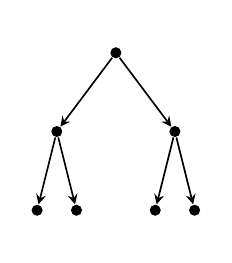
\begin{tikzpicture}[
		every label/.style={font=\scriptsize},
		state/.style={inner sep=0pt,fill,minimum size=4pt,circle,font=\scriptsize},
		arc/.style={->,>=stealth,semithick},
		probability/.style={-,densely dashed},
	]

\node at (1.25,1.2) {};
\node at (1.25,-1.2) {};
\node [state,label=] (s1) at (1.25,1.0) {};	

\node [inner sep=0pt,circle,fill,minimum size=4pt] (s1_1) at (0.5,0.0) {};
\node [inner sep=0pt,circle,fill,minimum size=4pt] (s1_2) at (2.0,0.0) {};

\node [inner sep=0pt,circle,fill,minimum size=4pt] (s1_3) at (0.25,-1.0) {};
\node [inner sep=0pt,circle,fill,minimum size=4pt] (s1_4) at (0.75,-1.0) {};
\node [inner sep=0pt,circle,fill,minimum size=4pt] (s1_5) at (1.75,-1.0) {};
\node [inner sep=0pt,circle,fill,minimum size=4pt] (s1_6) at (2.25,-1.0) {};


\draw [arc] (s1) to node [auto,pos=0.57,swap,font=\scriptsize] {} (s1_1);
\draw [arc] (s1) to node [auto,pos=0.57,font=\scriptsize] {} (s1_2);
\draw [arc] (s1_1) to node [auto,swap,font=\scriptsize,anchor=base east] {} (s1_3);
\draw [arc] (s1_1) to node [auto,font=\scriptsize,anchor=base west] {} (s1_4);
\draw [arc] (s1_2) to node [auto,swap,font=\scriptsize,anchor=base east] {} (s1_5);
\draw [arc] (s1_2) to node [auto,font=\scriptsize,anchor=base west] {} (s1_6);

	
	\end{tikzpicture}	
	\else
	\includegraphics{Pictures/max_comp_ptetbt_a}
	\fi
	
	&
	
	\ifwithtikz
\tikzsetnextfilename{max_comp_ptetbt_b}
	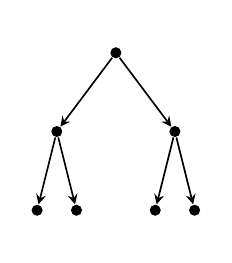
\begin{tikzpicture}[
		every label/.style={font=\scriptsize},
		state/.style={inner sep=0pt,fill,minimum size=4pt,circle,font=\scriptsize},
		arc/.style={->,>=stealth,semithick},
		probability/.style={-,densely dashed},
	]

\node at (1.25,1.2) {};
\node at (1.25,-1.2) {};
\node [state,label=] (s1) at (1.25,1.0) {};	

\node [inner sep=0pt,circle,fill,minimum size=4pt] (s1_1) at (0.5,0.0) {};
\node [inner sep=0pt,circle,fill,minimum size=4pt] (s1_2) at (2.0,0.0) {};

\node [inner sep=0pt,circle,fill,minimum size=4pt] (s1_3) at (0.25,-1.0) {};
\node [inner sep=0pt,circle,fill,minimum size=4pt] (s1_4) at (0.75,-1.0) {};
\node [inner sep=0pt,circle,fill,minimum size=4pt] (s1_5) at (1.75,-1.0) {};
\node [inner sep=0pt,circle,fill,minimum size=4pt] (s1_6) at (2.25,-1.0) {};


\draw [arc] (s1) to node [auto,pos=0.57,swap,font=\scriptsize] {} (s1_1);
\draw [arc] (s1) to node [auto,pos=0.57,font=\scriptsize] {} (s1_2);
\draw [arc] (s1_1) to node [auto,swap,font=\scriptsize,anchor=base east] {} (s1_3);
\draw [arc] (s1_1) to node [auto,font=\scriptsize,anchor=base west] {} (s1_4);
\draw [arc] (s1_2) to node [auto,swap,font=\scriptsize,anchor=base east] {} (s1_5);
\draw [arc] (s1_2) to node [auto,font=\scriptsize,anchor=base west] {} (s1_6);

	
	\end{tikzpicture}	
	\else
	\includegraphics{Pictures/max_comp_ptetbt_b}
	\fi
	
	&
	
	\ifwithtikz
\tikzsetnextfilename{max_comp_ptetbt_c}
	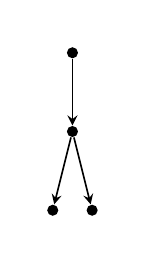
\begin{tikzpicture}[
		every label/.style={font=\scriptsize},
		state/.style={inner sep=0pt,fill,minimum size=4pt,circle,font=\scriptsize},
		arc/.style={->,>=stealth,semithick},
		probability/.style={-,densely dashed},
	]

\node at (1.25,1.2) {};
\node at (1.25,-1.2) {};
\node [state,label=] (s1) at (1.25,1.0) {};	

\node [inner sep=0pt,circle,fill,minimum size=4pt] (s1_1) at (1.25,0.0) {};

\node [inner sep=0pt,circle,fill,minimum size=4pt,label=left:] (s1_2) at (1.00,-1.0) {};
\node [inner sep=0pt,circle,fill,minimum size=4pt,label=right:] (s1_3) at (1.5,-1.0) {};


\draw [arc] (s1) to node [auto,pos=0.35,swap,font=\scriptsize] {} (s1_1);
\draw [arc] (s1_1) to node [auto,swap,font=\scriptsize,anchor=base east] {} (s1_2);
\draw [arc] (s1_1) to node [auto,font=\scriptsize,anchor=base west] {} (s1_3);

	
	\end{tikzpicture}
	\else
	\includegraphics{Pictures/max_comp_ptetbt_c}
	\fi
	
	&
	
	\ifwithtikz
\tikzsetnextfilename{max_comp_ptetbt_d}
	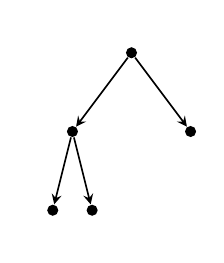
\begin{tikzpicture}[
		every label/.style={font=\scriptsize},
		state/.style={inner sep=0pt,fill,minimum size=4pt,circle,font=\scriptsize},
		arc/.style={->,>=stealth,semithick},
		probability/.style={-,densely dashed},
	]

\node at (1.25,1.2) {};
\node at (1.25,-1.2) {};
\node [state,label={}] (s1) at (1.25,1.0) {};	

\node [inner sep=0pt,circle,fill,minimum size=4pt] (s1_1) at (0.5,0.0) {};
\node [inner sep=0pt,circle,fill,minimum size=4pt] (s1_2) at (2.0,0.0) {};

\node [inner sep=0pt,circle,fill,minimum size=4pt,label=left:] (s1_3) at (0.25,-1.0) {};
\node [inner sep=0pt,circle,fill,minimum size=4pt,label=right:] (s1_4) at (0.75,-1.0) {};



\draw [arc] (s1) to node [auto,pos=0.57,swap,font=\scriptsize] {} (s1_1);
\draw [arc] (s1) to node [auto,pos=0.57,font=\scriptsize] {} (s1_2);
\draw [arc] (s1_1) to node [auto,swap,font=\scriptsize,anchor=base east] {} (s1_3);
\draw [arc] (s1_1) to node [auto,font=\scriptsize,anchor=base west] {} (s1_4);


	
	\end{tikzpicture}	
	\else
	\includegraphics{Pictures/max_comp_ptetbt_d}
	\fi
	
	&
	
	\ifwithtikz
\tikzsetnextfilename{max_comp_ptetbt_e}
	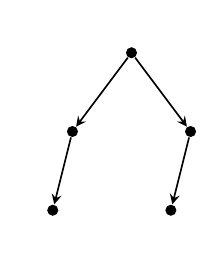
\begin{tikzpicture}[
		every label/.style={font=\scriptsize},
		state/.style={inner sep=0pt,fill,minimum size=4pt,circle,font=\scriptsize},
		arc/.style={->,>=stealth,semithick},
		probability/.style={-,densely dashed},
	]

\node at (1.25,1.2) {};
\node at (1.25,-1.2) {};
\node [state,label={}] (s1) at (1.25,1.0) {};	

\node [inner sep=0pt,circle,fill,minimum size=4pt] (s1_1) at (0.5,0.0) {};
\node [inner sep=0pt,circle,fill,minimum size=4pt] (s1_2) at (2.0,0.0) {};

\node [inner sep=0pt,circle,fill,minimum size=4pt,label=left:] (s1_3) at (0.25,-1.0) {};
\node [inner sep=0pt,circle,fill,minimum size=4pt,label=right:] (s1_5) at (1.75,-1.0) {};



\draw [arc] (s1) to node [auto,pos=0.57,swap,font=\scriptsize] {} (s1_1);
\draw [arc] (s1) to node [auto,pos=0.57,font=\scriptsize] {} (s1_2);
\draw [arc] (s1_1) to node [auto,swap,font=\scriptsize,anchor=base east] {} (s1_3);
\draw [arc] (s1_2) to node [auto,swap,font=\scriptsize,anchor=base east] {} (s1_5);


	
	\end{tikzpicture}	
	\else
	\includegraphics{Pictures/max_comp_ptetbt_e}
	\fi

	\\
	
		\multicolumn{2}{c}{
	\emph{\small processes}
	}
 & \emph{\small test} &
	\multicolumn{2}{c}{
	\emph{\small interaction systems}	
	}
	
	\end{tabular}
	\end{center}
 \caption{NPLTS models distinguished by  thanks to the restriction to
}
\label{fig:max_comp_ptetbt}

	\end{figure}

We now investigate the inclusion and compatibility properties of
/. Similar to
, they result in a testing semantics finer than trace semantics.

	\begin{thm}\label{thm:ptetbt_incl_ptr}

Let  be an NPLTS and . Then:
\cws{12}{\begin{array}{rcl}
s_{1} \sbis{\textrm{\rm PTe-tbt}} s_{2} & \!\!\! \Longrightarrow \!\!\! & s_{1} \sbis{\rm PTr} s_{2} \\
s_{1} \sbis{\textrm{\rm PTe-tbt}}^{\rm ct} s_{2} & \!\!\! \Longrightarrow \!\!\! & s_{1} \sbis{\rm PTr}^{\rm
ct} s_{2} \\
\end{array}}

\proof
If , then in particular for every NPT  with initial state  having a single maximal computation that is
labeled with  and reaches success, it holds that:

		\begin{itemize}

\item For each  there exists  such that:
\cws{10}{\hspace*{-1.2cm} \ms{prob}(\calscc(z_{s_{1}, o}, \alpha)) \: = \: \ms{prob}(\calscc(z_{s_{2}, o},
\alpha))}

\item For each  there exists  such that:
\cws{10}{\hspace*{-1.2cm} \ms{prob}(\calscc(z_{s_{2}, o}, \alpha)) \: = \: \ms{prob}(\calscc(z_{s_{1}, o},
\alpha))}

		\end{itemize}

\noindent
Since  for all  due to the structure of  -- where  and
 originates  in the interaction with  -- we immediately
derive that for all  it holds that:

		\begin{itemize}

\item For each  there exists  such that:
\cws{10}{\hspace*{-1.2cm} \ms{prob}(\calcc(z_{s_{1}}, \alpha)) \: = \: \ms{prob}(\calcc(z_{s_{2}}, \alpha))}

\item For each  there exists  such that:
\cws{10}{\hspace*{-1.2cm} \ms{prob}(\calcc(z_{s_{2}}, \alpha)) \: = \: \ms{prob}(\calcc(z_{s_{1}}, \alpha))}

		\end{itemize}

\noindent
This means that . \\
The proof of  is analogous.
\qed 

	\end{thm}

The inclusion of  (resp.\ ) in 
(resp.\ ) is strict. For instance, the two NPLTS models in
Fig.~\ref{fig:counterex_pteallexists_trace} are not trace-by-trace testing equivalent. In fact, the test in
the same figure distinguishes  from  because -- looking at the two interaction systems in
Fig.~\ref{fig:counterex_pteallexists_trace} -- each of the two maximal resolutions of  has a
maximal computation labeled with  while the only maximal resolution of  has not.

Unlike  and ,
/ result in a testing semantics that is
\emph{fully} (i.e., regardless of admitted tests) backward compatible with , , and . Concerning the two restricted classes of probabilistic processes, it is
worth recalling that bisimulation equivalence and trace equivalence were defined uniformly for fully
probabilistic processes~\cite{GJS90,JS90} and reactive probabilistic processes~\cite{LS91,Sei95}. In
contrast, testing equivalence for fully probabilistic processes was defined in~\cite{Chr90,CDSY99} in a way
that resembles , while for reactive probabilistic processes it was
defined in~\cite{KN98} in a way similar to . Our compatibility results
thus show that also testing equivalence could have been defined uniformly for both classes of probabilistic
processes without internal nondeterminism, by resorting to the trace-by-trace approach that we have
developed for NPLTS models.

	\begin{thm}\label{thm:ptetbt_compat}

Let  be an NPLTS and .

		\begin{enumerate}

\item If  is fully nondeterministic, then:
\cws{10}{\hspace*{-1.2cm} s_{1} \sbis{\textrm{\rm PTe-tbt}} s_{2} \: \Longleftrightarrow \: s_{1}
\sbis{\textrm{\rm PTe-tbt}}^{\rm ct} s_{2} \: \Longleftrightarrow \: s_{1} \sbis{\rm Te,fnd} s_{2}}

\item If  is fully probabilistic, then:
\cws{10}{\hspace*{-1.2cm} s_{1} \sbis{\textrm{\rm PTe-tbt}} s_{2} \: \Longleftrightarrow \: s_{1}
\sbis{\textrm{\rm PTe-tbt}}^{\rm ct} s_{2} \: \Longleftrightarrow \: s_{1} \sbis{\rm Tr,fpr} s_{2}}

\item If  is reactive probabilistic, then:
\cws{10}{\hspace*{-1.2cm}\begin{array}{rcl}
s_{1} \sbis{\textrm{\rm PTe-tbt}} s_{2} & \!\!\! \Longrightarrow \!\!\! & s_{1} \sbis{\rm Tr,rpr} s_{2} \\
s_{1} \sbis{\textrm{\rm PTe-tbt}}^{\rm ct} s_{2} & \!\!\! \Longrightarrow \!\!\! & s_{1} \sbis{\rm Tr,rpr}
s_{2} \\
\end{array}}

		\end{enumerate}

\proof
We proceed as follows:

		\begin{enumerate}

\item Suppose that  is fully nondeterministic. We recall from~\cite{DH84} that  means that for every \emph{fully nondeterministic} NPT  with initial state  it holds that:

			\begin{itemize}

\item There exists a successful computation from  iff there exists a successful computation from
.

\item All maximal computations from  are successful iff all maximal computations from  are successful.

			\end{itemize}

\noindent
In this setting, randomized schedulers are not important because, due to the absence of probabilistic
choices, the model cannot contain submodels that arise from convex combinations of other submodels. Thus, we
can concentrate on . Suppose that . Then, in
particular, for every \emph{fully nondeterministic} NPT  with initial
state  and for all  it holds that:

			\begin{itemize}

\item For each  there exists  such that:
\cws{10}{\hspace*{-2.4cm} \ms{prob}(\calscc(z_{s_{1}, o}, \alpha)) \: = \: \ms{prob}(\calscc(z_{s_{2}, o},
\alpha))}

\item For each  there exists  such that:
\cws{10}{\hspace*{-2.4cm} \ms{prob}(\calscc(z_{s_{2}, o}, \alpha)) \: = \: \ms{prob}(\calscc(z_{s_{1}, o},
\alpha))}

			\end{itemize}

\noindent
Since the NPLTS under test and the considered tests are all fully nondeterministic, the resulting
interaction systems are fully nondeterministic too, and hence their maximal resolutions coincide with their
maximal computations and each of the probability values above is either  or . As a consequence, the
previous relationships among maximal resolutions can be rephrased as follows:

			\begin{itemize}

\item For each maximal -compatible computation from  there exists a maximal
-compatible computation from  such that the two computations are both successful or both
unsuccessful.

\item For each maximal -compatible computation from  there exists a maximal
-compatible computation from  such that the two computations are both successful or both
unsuccessful.

			\end{itemize}

\noindent
From this, we immediately derive that:

			\begin{itemize}

\item There exists a successful computation from  iff there exists a successful computation from
.

\item All maximal computations from  are successful iff all maximal computations from  are successful. In fact, assume that all maximal computations from, e.g.,  are successful.
Then at least one maximal computation from  is successful. Assume that  has at least
two maximal computations and that one of them is not successful. Then at least one maximal computation from
 would not be successful, thus contradicting the assumption that all maximal computations from
 are successful. Therefore, whenever all maximal computations from  are successful,
then all maximal computations from  are successful. Likewise, whenever all maximal computations
from  are successful, then all maximal computations from  are successful.

			\end{itemize}

\noindent
This means that . \\
Suppose now that  and consider an \emph{arbitrary} NPT  with initial state , an arbitrary trace  such that
, and an arbitrary resolution . \\
Assume that , i.e., assume that for all  it holds that . Let
 be a \emph{fully nondeterministic} NPT obtained
from  in which (i)~only the maximal -compatible computations reach  and (ii)~each
transition  such that the set  has
cardinality greater than  is transformed into  transitions , , where  and  for all . Observing that  yields the same -compatible computations as
 in the interaction systems, the test  would violate 
because at least one maximal computation from  is successful whilst there are no maximal
computations from  that are successful. We have thus deduced that, whenever , then the existence of  implies the
existence of . \\
Assume now that for all  it holds that:
\cws{0}{\hspace*{-1.2cm} \ms{prob}(\calscc(z_{s_{1}, o}, \alpha)) \: \neq \: \ms{prob}(\calscc(z_{s_{2}, o},
\alpha))}
Observing that  must have a successful -compatible computation -- otherwise it would hold
that  for all
 -- from  and  we derive that
 and . Denoting
by  the element of  that originates , we would then have
that for each  originating :
\cws{0}{\hspace*{-1.2cm}\begin{array}{rcccl}
\ms{prob}(\calcc(z'_{s_{1}}, \alpha)) & \!\!\! = \!\!\! & \ms{prob}(\calscc(z_{s_{1}, o}, \alpha)) / p &
\!\!\! \neq \!\!\! & \\
& \!\!\! \neq \!\!\! & \ms{prob}(\calscc(z_{s_{2}, o}, \alpha)) / p & \!\!\! = \!\!\! &
\ms{prob}(\calcc(z'_{s_{2}}, \alpha)) \\
\end{array}}
where  is the probability of performing a successful -compatible computation in the element
 of  that originates . However, since the NPLTS under test is fully
nondeterministic,  and  boil down to two -compatible computations and it
holds that:
\cws{0}{\hspace*{-1.2cm} \ms{prob}(\calcc(z'_{s_{1}}, \alpha)) \: = \: 1 \: = \:
\ms{prob}(\calcc(z'_{s_{2}}, \alpha))}
which contradicts what established before. \\
In conclusion, whenever , then for each  there exists  such that:
\cws{0}{\hspace*{-1.2cm} \ms{prob}(\calscc(z_{s_{1}, o}, \alpha)) \: = \: \ms{prob}(\calscc(z_{s_{2}, o},
\alpha))}
With a similar argument, we can prove that, whenever , then for each
 there exists  such that:
\cws{0}{\hspace*{-1.2cm} \ms{prob}(\calscc(z_{s_{2}, o}, \alpha)) \: = \: \ms{prob}(\calscc(z_{s_{1}, o},
\alpha))}
This means that .

\item Suppose that  is fully probabilistic. We recall from~\cite{CDSY99} that  means that for every \emph{fully probabilistic} NPT 
with initial state  it holds that:
\cws{0}{\hspace*{-1.2cm} \ms{prob}(\calsc(s_{1}, o)) \: = \: \ms{prob}(\calsc(s_{2}, o))}
In this setting, schedulers are not important because there is no nondeterminism. Thus, we can concentrate
on . Suppose that . Then, in particular, for
every \emph{fully probabilistic} NPT  with initial state 
and for all  it holds that:

			\begin{itemize}

\item For each  there exists  such that:
\cws{10}{\hspace*{-2.4cm} \ms{prob}(\calscc(z_{s_{1}, o}, \alpha)) \: = \: \ms{prob}(\calscc(z_{s_{2}, o},
\alpha))}

\item For each  there exists  such that:
\cws{10}{\hspace*{-2.4cm} \ms{prob}(\calscc(z_{s_{2}, o}, \alpha)) \: = \: \ms{prob}(\calscc(z_{s_{1}, o},
\alpha))}

			\end{itemize}

\noindent
Since the NPLTS under test and the considered tests are all fully probabilistic, the resulting interaction
systems are fully probabilistic too, and hence each of them has a single maximal resolution that coincides
with the interaction system itself. As a consequence, the previous relationships among maximal resolutions
can be rephrased by saying that for all :
\cws{0}{\hspace*{-1.2cm} \ms{prob}(\calscc((s_{1}, o), \alpha)) \: = \: \ms{prob}(\calscc((s_{2}, o),
\alpha))}
From this, we immediately derive that:
\cws{0}{\hspace*{-1.2cm}\begin{array}{rcccl}
\ms{prob}(\calsc(s_{1}, o)) & \!\!\! = \!\!\! & \sum\limits_{\alpha \in A^{*}} \ms{prob}(\calscc((s_{1}, o),
\alpha)) & \!\!\! = \!\!\! & \0.4cm]
\bigsqcap\limits_{\alpha \in \ms{Tr}_{\rm max}(s_{1}, o)} \ms{prob}(\calscc((s_{1}, o), \alpha)) & \!\!\! =
\!\!\! & \bigsqcap\limits_{\alpha \in \ms{Tr}_{\rm max}(s_{2}, o)} \ms{prob}(\calscc((s_{2}, o), \alpha)) \\
\end{array}}
Given , the set  contains all the traces labeling the maximal computations
from , while success probabilities  are viewed as being
conditional on selecting the maximal resolution of  that contains all the -compatible
computations from  (this resolution is unique because interaction systems are reactive
probabilistic). \\
Suppose that . Then, in particular, for every \emph{reactive
probabilistic} NPT  with initial state  and for all  it holds that:

			\begin{itemize}

\item For each  there exists  such that:
\cws{10}{\hspace*{-2.4cm} \ms{prob}(\calscc(z_{s_{1}, o}, \alpha)) \: = \: \ms{prob}(\calscc(z_{s_{2}, o},
\alpha))}

\item For each  there exists  such that:
\cws{10}{\hspace*{-2.4cm} \ms{prob}(\calscc(z_{s_{2}, o}, \alpha)) \: = \: \ms{prob}(\calscc(z_{s_{1}, o},
\alpha))}

			\end{itemize}

\noindent
Since the NPLTS under test and the considered tests are all reactive probabilistic, the resulting
interaction systems are reactive probabilistic too, and hence in each of them there is a unique maximal
resolution that collects all the computations compatible with a given maximal trace. As a consequence, from
the previous relationships among maximal resolutions we derive that for all :
\cws{0}{\hspace*{-1.2cm} \ms{prob}(\calscc((s_{1}, o), \alpha)) \: = \: \ms{prob}(\calscc((s_{2}, o),
\alpha))}
From this, we immediately derive that:
\cws{0}{\hspace*{-1.2cm}\begin{array}{rcl}
\bigsqcup\limits_{\alpha \in \ms{Tr}_{\rm max}(s_{1}, o)} \ms{prob}(\calscc((s_{1}, o), \alpha)) & \!\!\! =
\!\!\! & \bigsqcup\limits_{\alpha \in \ms{Tr}_{\rm max}(s_{2}, o)} \ms{prob}(\calscc((s_{2}, o), \alpha))
\0.1cm]
\hspace*{0.8cm} = \: \sum_{R'_{1}, \dots, R'_{n} \in 2^{A} \, {\rm s.t.} \, R'_{i} \cap F_{i} = \emptyset \,
{\rm for \hspace{0.08cm} all} \, i = 1, \dots, n} \ms{prob}(\calrtcc(z_{s_{2}}, (a_{1}, R'_{1}) \dots
(a_{n}, R'_{n}))) \0.1cm]
\hspace*{0.8cm} = \: \ms{prob}(\calftcc(z_{s_{2}}, (a_{1}, F_{1}) \dots (a_{n}, F_{n}))) \\
\end{array}}

\item Symmetrically for each .

		\end{itemize}

\noindent
This means that . \\
Thirdly, we prove that . Suppose that . Since for all , , , , and  it holds that:
\cws{0}{\ms{prob}(\calfcc(z_{s}, (\alpha, F))) \: = \: \ms{prob}(\calftcc(z_{s}, (a_{1}, \emptyset) \dots
(a_{n - 1}, \emptyset) (a_{n}, F)))}
we immediately derive that:

		\begin{itemize}

\item For each  there exists  such that for
all failure pairs :
\cws{0}{\hspace*{-1.2cm}\begin{array}{rcl}
\ms{prob}(\calfcc(z_{s_{1}}, (a_{1} \dots a_{n}, F))) & \!\!\! = \!\!\! & \ms{prob}(\calftcc(z_{s_{1}},
(a_{1}, \emptyset) \dots (a_{n - 1}, \emptyset) (a_{n}, F))) \\
& \!\!\! = \!\!\! & \ms{prob}(\calftcc(z_{s_{2}}, (a_{1}, \emptyset) \dots (a_{n - 1}, \emptyset) (a_{n},
F))) \\
& \!\!\! = \!\!\! & \ms{prob}(\calfcc(z_{s_{2}}, (a_{1} \dots a_{n}, F))) \\
\end{array}}

\item Symmetrically for each .

		\end{itemize}

\noindent
This means that .
\qed 

	\end{thm}

The inclusion of  in  is strict, because for the two NPLTS
models in Fig.~\ref{fig:counterex_tefnd_testing} it holds that  while  as witnessed by the test in the same figure (see the maximal
resolutions of the interaction systems in Fig.~\ref{fig:counterex_tefnd_testing_max_res}).

	\begin{thm}\label{thm:pfdis_incl_ptrdis}

Let  be an NPLTS and . Then:
\cws{10}{\begin{array}{rcl}
s_{1} \sbis{\rm PF,dis} s_{2} & \!\!\! \Longrightarrow \!\!\! & s_{1} \sbis{\rm PTr,dis} s_{2} \\
s_{1} \sbis{\rm PF,dis}^{\rm ct} s_{2} & \!\!\! \Longrightarrow \!\!\! & s_{1} \sbis{\rm PTr,dis}^{\rm ct}
s_{2} \\
\end{array}}

\proof
Suppose that . Then  because for all , , and  it holds that:
\cws{0}{\ms{prob}(\calcc(z_{s}, \alpha)) \: = \: \ms{prob}(\calfcc(z_{s}, (\alpha, \emptyset)))}
and hence:

		\begin{itemize}

\item For each  there exists  such that for
all :
\cws{0}{\hspace*{-1.2cm}\begin{array}{rcccl}
\ms{prob}(\calcc(z_{s_{1}}, \alpha)) & \!\!\! = \!\!\! & \ms{prob}(\calfcc(z_{s_{1}}, (\alpha, \emptyset)))
& \!\!\! = \!\!\! & \\
& \!\!\! = \!\!\! & \ms{prob}(\calfcc(z_{s_{2}}, (\alpha, \emptyset))) & \!\!\! = \!\!\! &
\ms{prob}(\calcc(z_{s_{2}}, \alpha)) \\
\end{array}}

\item Symmetrically for each .

		\end{itemize}

\noindent
The proof that  implies  is
similar.
\qed 

	\end{thm}

The inclusion of  (resp.\ ) in  (resp.\
) is strict, because the initial states of the two NPLTS models in
Fig.~\ref{fig:counterex_pteallexists_trace} are equated by the latter equivalence and told apart by the
former.

	\begin{thm}\label{thm:pf_incl_ptetbt}

Let  be an NPLTS and . Then:
\cws{10}{\begin{array}{rcl}
s_{1} \sbis{\rm PF} s_{2} & \!\!\! \Longrightarrow \!\!\! & s_{1} \sbis{\textrm{\rm PTe-tbt}} s_{2} \\
s_{1} \sbis{\rm PF}^{\rm ct} s_{2} & \!\!\! \Longrightarrow \!\!\! & s_{1} \sbis{\textrm{\rm PTe-tbt}}^{\rm
ct} s_{2} \\
\end{array}}

\proof
Let us prove the contrapositive of the first result, i.e., . Thus, suppose that . This means that there exist an NPT  with initial state , a trace , and, say, a resolution  such that  or for all  it holds that:
\cws{0}{\ms{prob}(\calscc(z_{s_{1}, o}, \alpha)) \: \neq \: \ms{prob}(\calscc(z_{s_{2}, o}, \alpha))}
Observing that , in the case that  either  cannot perform  at all -- let  -- or, after performing , the states reached by  can always synchronize
with the states reached by  on a set  of actions whereas the states reached by  cannot -- let
. The failure pair  shows that  in this case
because, denoting by  the element of  that originates~, we have that
for all :
\cws{0}{\ms{prob}(\calfcc(z'_{s_{1}}, \varphi)) \: > \: 0 \: = \: \ms{prob}(\calfcc(z'_{s_{2}}, \varphi))}
In the case that , the failure pair  shows that . In fact, without loss of generality we can
assume that the only -compatible computations in~ are the ones exercised by  --
note that they must belong to the same element  of  -- as the only effect of this
assumption is that of possibly reducing the number of resolutions in . At least one of these computations must be successful -- and hence maximal -- in~ because
otherwise the success probabilities of the considered resolutions would all be equal to~. Denoting by
 the element of  that originates~, we then have that for all
 originating some :
\cws{0}{\begin{array}{rcccl}
\ms{prob}(\calfcc(z'_{s_{1}}, \varphi)) & \!\!\! = \!\!\! & \ms{prob}(\calscc(z_{s_{1}, o}, \alpha)) / p &
\!\!\! \neq \!\!\! & \\
& \!\!\! \neq \!\!\! & \ms{prob}(\calscc(z_{s_{2}, o}, \alpha)) / p & \!\!\! = \!\!\! &
\ms{prob}(\calfcc(z'_{s_{2}}, \varphi)) \\
\end{array}}
where  is the probability of performing the -compatible computations in the only element 
of~ that originates  and all the resolutions . \\
The proof that  implies 
is similar.
\qed 

	\end{thm}

The inclusion of  (resp.\ ) in  (resp.\
) is strict, because the initial states of the two NPLTS models in
Fig.~\ref{fig:counterex_ptrdis_ptr} are equated by the latter equivalence and told apart by the former.
For instance, the rightmost maximal resolution of  has probability~ of performing a computation
compatible with the failure pair , whilst each of the two maximal resolutions of
 has probability~.

	\begin{figure}[tp]

\centerline{\includegraphics{Pictures/spectrum}}
\caption{The spectrum of testing, failure, and trace equivalences for NPLTS models}
\label{fig:spectrum}

	\end{figure}

The relationships among the various probabilistic testing, failure, and trace equivalences for NPLTS models
are summarized in Fig.~\ref{fig:spectrum}. Arrows represent the more-discriminating-than partial order,
equivalences close to each other coincide, and incomparability is denoted by the absence of (chains of)
arrows. The various relationships have been established in this paper, except for the arrow from
 to  that is due to~\cite{Seg96}.

We observe that  is incomparable not only with 
as established right before Thm.~\ref{thm:pteallexists_incl_ptetbt}, but also with ,
, , and . In fact, in
Fig.~\ref{fig:counterex_ptesupinf_trace} it holds that  while
, , ,
and . On the other hand, in Fig.~\ref{fig:counterex_tefnd_testing} it holds
that  while , , , and .

Likewise,  is incomparable not only with  as established right
after Thm.~\ref{thm:pfdis_incl_pf}, but also with , , and
. Indeed, in Fig.~\ref{fig:counterex_ptesupinf_trace} it holds that  while , , and . In contrast, in Fig.~\ref{fig:counterex_pfdis_pf} it holds
that  while , , and . Moreover,  is
incomparable with  and . In fact, in
Fig.~\ref{fig:counterex_pfdis_pf} it holds that  while  and . On the other hand, in
Fig.~\ref{fig:counterex_pteallexists_trace} it holds that  while
 and . Additionally,  is incomparable with  because in Fig.~\ref{fig:counterex_ptesupinf_trace} we
have that  and , whereas in
Fig.~\ref{fig:counterex_pteallexists_trace} we have that  and . Furthermore,  is incomparable also with
 because in Fig.~\ref{fig:counterex_ptesupinf_trace} we have that  and , whilst in
Fig.~\ref{fig:counterex_ptrdis_ptr} we have that  and .

Analogously,  is incomparable not only with  as established
right after Thm.~\ref{thm:ptrdis_incl_ptr}, but also with , , and
. It holds that  and , , and  in Fig.~\ref{fig:counterex_pteallexists_trace}, while  and , , and  in Fig.~\ref{fig:counterex_pfdis_pf}. The same
two figures show that also  is incomparable with ,
, and . Finally, we have that  is
incomparable with  because in Fig.~\ref{fig:counterex_pteallexists_trace}
it holds that  and , whereas
in Fig.~\ref{fig:counterex_ptesupinf_trace} it holds that  and .

We conclude by recalling another probabilistic testing equivalence that has been recently proposed
in~\cite{GA12}, where a probabilistic model significantly different from ours is considered. Unfortunately,
the differences prevent us from placing that equivalence in the spectrum we have just presented. However,
that testing equivalence shares with our  motivations and intuitions concerning the
power of schedulers and the estimation of success probabilities that call for further comments.

The model considered in~\cite{GA12} has three types of transitions: action transitions, internal
transitions, and probabilistic transitions. Since each state can have only one type of outgoing transitions,
also states are divided into three classes: action states, nondeterministic states, and probabilistic
states. Action states cannot have two identically labeled action transitions, so this model can be viewed as
a variant of reactive probabilistic processes in which states of different classes can alternate along a
computation. Notice that our NPLTS model is non-alternating, because there is a single class of states and
probabilistic choices are somehow embedded within each single transition.

In order to make the proposed testing theory insensitive to the exact moment in which internal choices
occur, in~\cite{GA12} internal transitions are decorated with so-called internal labels. Similar to action
states, nondeterministic states cannot have two identically labeled internal transitions. Moreover, given
two nondeterministic states, either they share the same set of internal labels decorating their outgoing
transitions, or the sets of internal labels of their outgoing transitions are disjoint. Internal labels are
meant to provide precisely the information that schedulers should use to resolve internal choices, so that
internal choices relying on the same information are resolved in the same way. For example, continuing the
discussion done in the last two paragraphs of Sect.~\ref{sec:testing_equiv}, with the approach
of~\cite{GA12} the two internal choices between the two -transitions in the interaction system with
initial configuration  of Figs.~\ref{fig:counterex_tefnd_testing}
and~\ref{fig:counterex_tepr_testing} would be identically tagged, say with  and~ based on the
orientation of the arrows. As a consequence, the only allowed maximal resolutions of that interaction system
among the four shown in Figs.~\ref{fig:counterex_tefnd_testing_max_res}
and~\ref{fig:counterex_tepr_testing_max_res} would be the first one (choice of ) and the fourth one
(choice of~), thus excluding success probabilities~ and~.

An important technical point made in~\cite{GA12} is that, in the presence of cycles of transitions within
the model, the same internal choice may occur several times along a computation. This is not due to the
copying capability that arises when composing in parallel a process and a test, which -- as we have recalled
above -- is dealt with by labeling in the same way the internal transitions departing from all the copies of
the cloned state and by forcing schedulers to perform consistent choices in all the copies (we will refer to
the resulting fully probabilistic models as \emph{consistent resolutions}). Replications of the same
internal choice at different \emph{unfolding depths} of a cycle are independent of each other and are thus
given additional labels that keep them distinct from depth to depth. Notice that, in contrast, our approach
based on  is not invasive at all, as it does not require any label massaging on the
model to restrict the power of schedulers.

	\begin{figure}[tp]

	\begin{center}

	\begin{tabular}{cc@{\hspace{0.5cm}}c@{\hspace{0.5cm}}cc}

	\ifwithtikz
\tikzsetnextfilename{counterex_ptetbt_ga_a}	
	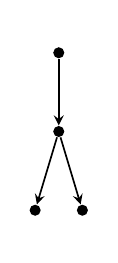
\begin{tikzpicture}[
		every label/.style={font=\scriptsize},
		state/.style={inner sep=0pt,fill,minimum size=4pt,circle,font=\scriptsize},
		arc/.style={->,>=stealth,semithick},
		probability/.style={-,densely dashed},
	]

\node at (1.5,1.2) {};
\node at (1.5,-1.2) {};
\node [state,label=] (s1) at (1.5,1.0) {};	

\node [inner sep=0pt,circle,fill,minimum size=4pt] (s1_1) at (1.5,0.0) {};

\node [inner sep=0pt,circle,fill,minimum size=4pt] (s1_2) at (1.2,-1.0) {};
\node [inner sep=0pt,circle,fill,minimum size=4pt] (s1_3) at (1.8,-1.0) {};




\draw [arc] (s1) to node [auto,pos=0.35,swap,font=\scriptsize] {} (s1_1);
\draw [arc] (s1_1) to node [font=\scriptsize,anchor=base east] {} (s1_2);
\draw [arc] (s1_1) to node [font=\scriptsize,anchor=base west] {} (s1_3);


	
	\end{tikzpicture}	
	\else
	\includegraphics{Pictures/counterex_ptetbt_ga_a}
	\fi
	
	&

	\ifwithtikz
\tikzsetnextfilename{counterex_ptetbt_ga_b}
	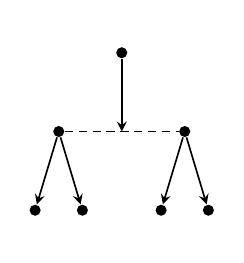
\begin{tikzpicture}[
		every label/.style={font=\scriptsize},
		state/.style={inner sep=0pt,fill,minimum size=4pt,circle,font=\scriptsize},
		arc/.style={->,>=stealth,semithick},
		probability/.style={-,densely dashed},
	]

\node at (1.5,1.2) {};
\node at (1.5,-1.2) {};
\node [state,label=] (s2) at (1.5,1.0) {};	

\node [inner sep=0pt,circle,fill,minimum size=4pt,label=] (s2_1) at (0.7,0.0) {};
\node [inner sep=0pt,circle,fill,minimum size=4pt,label=] (s2_2) at (2.3,0.0) {};

\node [inner sep=0pt,circle,fill,minimum size=4pt] (s2_3) at (0.4,-1.0) {};
\node [inner sep=0pt,circle,fill,minimum size=4pt] (s2_4) at (1.0,-1.0) {};

\node [inner sep=0pt,circle,fill,minimum size=4pt] (s2_5) at (2.0,-1.0) {};
\node [inner sep=0pt,circle,fill,minimum size=4pt] (s2_6) at (2.6,-1.0) {};

\draw [probability] (s2_1) -- (s2_2);

\draw [arc] (s2) to node [auto,pos=0.35,swap,font=\scriptsize] {} (1.5,0.0);

\draw [arc] (s2_1) to node [auto,swap,font=\scriptsize,anchor=base east] {}  (s2_3);
\draw [arc] (s2_1) to node [auto,font=\scriptsize,anchor=base west] {} (s2_4);

\draw [arc] (s2_2) to node [auto,swap,font=\scriptsize,anchor=base east] {}  (s2_5);
\draw [arc] (s2_2) to node [auto,font=\scriptsize,anchor=base west] {}  (s2_6);

	
	\end{tikzpicture}	
	\else
	\includegraphics{Pictures/counterex_ptetbt_ga_b}
	\fi
	
	&

	\ifwithtikz
\tikzsetnextfilename{counterex_ptetbt_ga_c}
	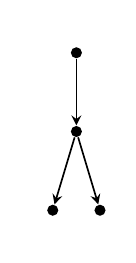
\begin{tikzpicture}[
		every label/.style={font=\scriptsize},
		state/.style={inner sep=0pt,fill,minimum size=4pt,circle,font=\scriptsize},
		arc/.style={->,>=stealth,semithick},
		probability/.style={-,densely dashed},
	]

\node at (1.5,1.2) {};
\node at (1.5,-1.2) {};
\node [state,label=] (s1) at (1.5,1.0) {};	

\node [inner sep=0pt,circle,fill,minimum size=4pt] (s1_1) at (1.5,0.0) {};

\node [inner sep=0pt,circle,fill,minimum size=4pt,label=left:] (s1_2) at (1.2,-1.0) {};
\node [inner sep=0pt,circle,fill,minimum size=4pt] (s1_3) at (1.8,-1.0) {};




\draw [arc] (s1) to node [auto,pos=0.35,swap,font=\scriptsize] {} (s1_1);
\draw [arc] (s1_1) to node [font=\scriptsize,anchor=base east] {} (s1_2);
\draw [arc] (s1_1) to node [font=\scriptsize,anchor=base west] {} (s1_3);


	\end{tikzpicture}
	\else
	\includegraphics{Pictures/counterex_ptetbt_ga_c}
	\fi
	
	&

	\ifwithtikz
\tikzsetnextfilename{counterex_ptetbt_ga_d}
	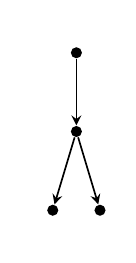
\begin{tikzpicture}[
		every label/.style={font=\scriptsize},
		state/.style={inner sep=0pt,fill,minimum size=4pt,circle,font=\scriptsize},
		arc/.style={->,>=stealth,semithick},
		probability/.style={-,densely dashed},
	]

\node at (1.5,1.2) {};
\node at (1.5,-1.2) {};
\node [state,label={}] (s1) at (1.5,1.0) {};	

\node [inner sep=0pt,circle,fill,minimum size=4pt] (s1_1) at (1.5,0.0) {};

\node [inner sep=0pt,circle,fill,minimum size=4pt,label=left:] (s1_2) at (1.2,-1.0) {};
\node [inner sep=0pt,circle,fill,minimum size=4pt] (s1_3) at (1.8,-1.0) {};




\draw [arc] (s1) to node [auto,pos=0.35,swap,font=\scriptsize] {} (s1_1);
\draw [arc] (s1_1) to node [font=\scriptsize,anchor=base east] {} (s1_2);
\draw [arc] (s1_1) to node [font=\scriptsize,anchor=base west] {} (s1_3);


	\end{tikzpicture}
	\else
	\includegraphics{Pictures/counterex_ptetbt_ga_d}
	\fi
	
	&

	\ifwithtikz
\tikzsetnextfilename{counterex_ptetbt_ga_e}
	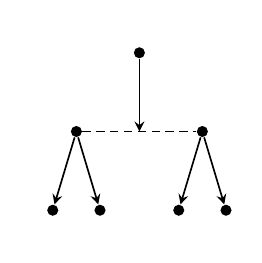
\begin{tikzpicture}[
		every label/.style={font=\scriptsize},
		state/.style={inner sep=0pt,fill,minimum size=4pt,circle,font=\scriptsize},
		arc/.style={->,>=stealth,semithick},
		probability/.style={-,densely dashed},
	]

\node at (1.5,1.2) {};
\node at (1.5,-1.2) {};
\node [state,label={}] (s2) at (1.5,1.0) {};	

\node [inner sep=0pt,circle,fill,minimum size=4pt,label=] (s2_1) at (0.7,0.0) {};
\node [inner sep=0pt,circle,fill,minimum size=4pt,label=] (s2_2) at (2.3,0.0) {};

\node [inner sep=0pt,circle,fill,minimum size=4pt,label=left:] (s2_3) at (0.4,-1.0) {};
\node [inner sep=0pt,circle,fill,minimum size=4pt] (s2_4) at (1.0,-1.0) {};

\node [inner sep=0pt,circle,fill,minimum size=4pt,label=left:] (s2_5) at (2.0,-1.0) {};
\node [inner sep=0pt,circle,fill,minimum size=4pt] (s2_6) at (2.6,-1.0) {};

\draw [probability] (s2_1) -- (s2_2);

\draw [arc] (s2) to node [auto,pos=0.35,swap,font=\scriptsize] {} (1.5,0.0);

\draw [arc] (s2_1) to node [auto,swap,font=\scriptsize,anchor=base east] {}  (s2_3);
\draw [arc] (s2_1) to node [auto,font=\scriptsize,anchor=base west] {} (s2_4);

\draw [arc] (s2_2) to node [auto,swap,font=\scriptsize,anchor=base east] {}  (s2_5);
\draw [arc] (s2_2) to node [auto,font=\scriptsize,anchor=base west] {}  (s2_6);

	
	
	\end{tikzpicture} 
		\else
	\includegraphics{Pictures/counterex_ptetbt_ga_e}
	\fi
	\\
	
		\multicolumn{2}{c}{
	\emph{\small processes}
	}
 & \emph{\small test} &
	\multicolumn{2}{c}{
	\emph{\small interaction systems}	
	}

	\end{tabular}
	\end{center}
 \caption{NPLTS models equated by~\cite{GA12} and distinguished by }
\label{fig:counterex_ptetbt_ga}

	\end{figure}

	\begin{figure}

	\begin{center}
	
		\begin{tabular}{cccccc}

	\ifwithtikz
\tikzsetnextfilename{counterex_ptetbt_ga_max_res_a}
	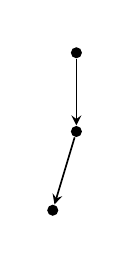
\begin{tikzpicture}[
		every label/.style={font=\scriptsize},
		state/.style={inner sep=0pt,fill,minimum size=4pt,circle,font=\scriptsize},
		arc/.style={->,>=stealth,semithick},
		probability/.style={-,densely dashed},
	]

\node at (1.5,1.2) {};
\node at (1.5,-1.2) {};
\node [state,label={}] (s1) at (1.5,1.0) {};	

\node [inner sep=0pt,circle,fill,minimum size=4pt] (s1_1) at (1.5,0.0) {};

\node [inner sep=0pt,circle,fill,minimum size=4pt,label=left:] (s1_2) at (1.2,-1.0) {};





\draw [arc] (s1) to node [auto,pos=0.35,swap,font=\scriptsize] {} (s1_1);
\draw [arc] (s1_1) to node [font=\scriptsize,anchor=base east] {} (s1_2);


	\end{tikzpicture}
	\else
	\includegraphics{Pictures/counterex_ptetbt_ga_max_res_a}
	\fi
	
	&

	\ifwithtikz
\tikzsetnextfilename{counterex_ptetbt_ga_max_res_b}
	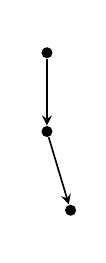
\begin{tikzpicture}[
		every label/.style={font=\scriptsize},
		state/.style={inner sep=0pt,fill,minimum size=4pt,circle,font=\scriptsize},
		arc/.style={->,>=stealth,semithick},
		probability/.style={-,densely dashed},
	]

\node at (1.5,1.2) {};
\node at (1.5,-1.2) {};
\node [state,label={}] (s1) at (1.5,1.0) {};	

\node [inner sep=0pt,circle,fill,minimum size=4pt] (s1_1) at (1.5,0.0) {};

\node [inner sep=0pt,circle,fill,minimum size=4pt] (s1_3) at (1.8,-1.0) {};




\draw [arc] (s1) to node [auto,pos=0.35,swap,font=\scriptsize] {} (s1_1);
\draw [arc] (s1_1) to node [font=\scriptsize,anchor=base west] {} (s1_3);


	
	\end{tikzpicture}
	\else
	\includegraphics{Pictures/counterex_ptetbt_ga_max_res_b}
	\fi
	
	&

	\ifwithtikz
\tikzsetnextfilename{counterex_ptetbt_ga_max_res_c}
	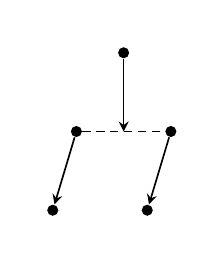
\begin{tikzpicture}[
		every label/.style={font=\scriptsize},
		state/.style={inner sep=0pt,fill,minimum size=4pt,circle,font=\scriptsize},
		arc/.style={->,>=stealth,semithick},
		probability/.style={-,densely dashed},
	]

\node at (1.5,1.2) {};
\node at (1.5,-1.2) {};
\node [state,label={}] (s2) at (1.5,1.0) {};	

\node [inner sep=0pt,circle,fill,minimum size=4pt,label=] (s2_1) at (0.9,0.0) {};
\node [inner sep=0pt,circle,fill,minimum size=4pt,label=] (s2_2) at (2.1,0.0) {};

\node [inner sep=0pt,circle,fill,minimum size=4pt,label=left:] (s2_3) at (0.6,-1.0) {};


\node [inner sep=0pt,circle,fill,minimum size=4pt,label=left:] (s2_5) at (1.8,-1.0) {};


\draw [probability] (s2_1) -- (s2_2);

\draw [arc] (s2) to node [auto,pos=0.35,swap,font=\scriptsize] {} (1.5,0.0);

\draw [arc] (s2_1) to node [auto,swap,font=\scriptsize,anchor=base east] {}  (s2_3);


\draw [arc] (s2_2) to node [auto,swap,font=\scriptsize,anchor=base east] {}  (s2_5);


	
	
	\end{tikzpicture}
	\else
	\includegraphics{Pictures/counterex_ptetbt_ga_max_res_c}
	\fi
	
	&

	\ifwithtikz
\tikzsetnextfilename{counterex_ptetbt_ga_max_res_d}
	\begin{tikzpicture}[
		every label/.style={font=\scriptsize},
		state/.style={inner sep=0pt,fill,minimum size=4pt,circle,font=\scriptsize},
		arc/.style={->,>=stealth,semithick},
		probability/.style={-,densely dashed},
	]

\node at (1.5,1.2) {};
\node at (1.5,-1.2) {};
\node [state,label={}] (s2) at (1.5,1.0) {};	

\node [inner sep=0pt,circle,fill,minimum size=4pt,label=] (s2_1) at (0.9,0.0) {};
\node [inner sep=0pt,circle,fill,minimum size=4pt,label=] (s2_2) at (2.1,0.0) {};

\node [inner sep=0pt,circle,fill,minimum size=4pt,label=left:] (s2_3) at (0.6,-1.0) {};


\node [inner sep=0pt,circle,fill,minimum size=4pt] (s2_6) at (2.4,-1.0) {};

\draw [probability] (s2_1) -- (s2_2);

\draw [arc] (s2) to node [auto,pos=0.35,swap,font=\scriptsize] {} (1.5,0.0);

\draw [arc] (s2_1) to node [auto,swap,font=\scriptsize,anchor=base east] {}  (s2_3);


\draw [arc] (s2_2) to node [auto,font=\scriptsize,anchor=base west] {}  (s2_6);

	
	
	\end{tikzpicture}
	\else
	\includegraphics{Pictures/counterex_ptetbt_ga_max_res_d}
	\fi
	
	&

	\ifwithtikz
\tikzsetnextfilename{counterex_ptetbt_ga_max_res_e}
	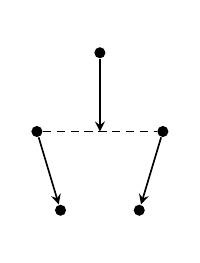
\begin{tikzpicture}[
		every label/.style={font=\scriptsize},
		state/.style={inner sep=0pt,fill,minimum size=4pt,circle,font=\scriptsize},
		arc/.style={->,>=stealth,semithick},
		probability/.style={-,densely dashed},
	]

\node at (1.5,1.2) {};
\node at (1.5,-1.2) {};
\node [state,label={}] (s2) at (1.5,1.0) {};	

\node [inner sep=0pt,circle,fill,minimum size=4pt,label=] (s2_1) at (0.7,0.0) {};
\node [inner sep=0pt,circle,fill,minimum size=4pt,label=] (s2_2) at (2.3,0.0) {};

\node [inner sep=0pt,circle,fill,minimum size=4pt] (s2_4) at (1.0,-1.0) {};

\node [inner sep=0pt,circle,fill,minimum size=4pt,label=left:] (s2_5) at (2.0,-1.0) {};


\draw [probability] (s2_1) -- (s2_2);

\draw [arc] (s2) to node [auto,pos=0.35,swap,font=\scriptsize] {} (1.5,0.0);

\draw [arc] (s2_1) to node [auto,font=\scriptsize,anchor=base west] {} (s2_4);

\draw [arc] (s2_2) to node [auto,swap,font=\scriptsize,anchor=base east] {}  (s2_5);



	
	\end{tikzpicture}
	\else
	\includegraphics{Pictures/counterex_ptetbt_ga_max_res_e}
	\fi
	
	&

	\ifwithtikz
\tikzsetnextfilename{counterex_ptetbt_ga_max_res_f}
	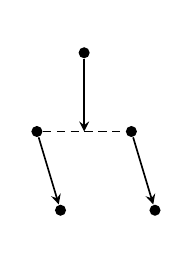
\begin{tikzpicture}[
		every label/.style={font=\scriptsize},
		state/.style={inner sep=0pt,fill,minimum size=4pt,circle,font=\scriptsize},
		arc/.style={->,>=stealth,semithick},
		probability/.style={-,densely dashed},
	]

\node at (1.5,1.2) {};
\node at (1.5,-1.2) {};
\node [state,label={}] (s2) at (1.5,1.0) {};	

\node [inner sep=0pt,circle,fill,minimum size=4pt,label=] (s2_1) at (0.9,0.0) {};
\node [inner sep=0pt,circle,fill,minimum size=4pt,label=] (s2_2) at (2.1,0.0) {};

\node [inner sep=0pt,circle,fill,minimum size=4pt] (s2_4) at (1.2,-1.0) {};

\node [inner sep=0pt,circle,fill,minimum size=4pt] (s2_6) at (2.4,-1.0) {};

\draw [probability] (s2_1) -- (s2_2);

\draw [arc] (s2) to node [auto,pos=0.35,swap,font=\scriptsize] {} (1.5,0.0);

\draw [arc] (s2_1) to node [auto,font=\scriptsize,anchor=base west] {} (s2_4);

\draw [arc] (s2_2) to node [auto,font=\scriptsize,anchor=base west] {}  (s2_6);

	
	
	\end{tikzpicture}
	\else
	\includegraphics{Pictures/counterex_ptetbt_ga_max_res_f}
	\fi
	
	\end{tabular}
	\end{center}
 \caption{Maximal resolutions of the two interaction systems in Fig.~\ref{fig:counterex_ptetbt_ga}}
\label{fig:counterex_ptetbt_ga_max_res}

	\end{figure}

Two processes are equated by the testing equivalence proposed in~\cite{GA12} iff, for each test, every
consistent resolution at unfolding depth  of a suitably labeled version of the first interaction system
that reaches success with probability , is matched by a consistent resolution at the same unfolding depth
of a suitably labeled version of the second interaction system that reaches success with the same
probability. This equivalence cannot be directly applied to NPLTS models. Since a major difference with
 is the use of restricted schedulers, an adaptation of the testing equivalence
of~\cite{GA12} to a common model should lead to an equivalence that is coarser than
.

It can however be shown that the two equivalences are different if attention is restricted to a common
submodel that does not permit internal nondeterminism. Indeed, absence of internal nondeterminism makes
label massaging unnecessary, and we have that reactive probabilistic processes constitute the largest
submodel common to the model of~\cite{GA12} and NPLTS. Consider the two reactive probabilistic processes
depicted as NPLTS models in Fig.~\ref{fig:counterex_ptetbt_ga}, and suppose that what is called
synchronization nondeterminism in~\cite{GA12} is handled without using  inside the labels of the
transitions of the interaction systems. The two processes are discriminated by 
because, if we consider the test in the same figure and the maximal resolutions shown in
Fig.~\ref{fig:counterex_ptetbt_ga_max_res} of the interaction systems, the success probability  of
trace  in the second maximal resolution of  is not matched by the success probability
 of the only maximal resolution of  having a maximal computation labeled with . In
contrast, the testing equivalence of~\cite{GA12} cannot distinguish the two processes. \linebreak Whenever
they remain in the interaction system with an arbitrary test, the two identical choices between  and 
in the second process must be resolved in the same way by any restricted scheduler that can only yield
consistent resolutions. For instance, the only maximal resolutions of  that are consistent among
the four shown in Fig.~\ref{fig:counterex_ptetbt_ga_max_res} are the first one (choice of ) and the
fourth one (choice of~), and their respective success probabilities  and  are precisely matched by
those of the only two maximal resolutions of .







\section{Conclusion}
\label{sec:concl}


In this paper, we have proposed two variants of trace and testing equivalences, respectively denoted by
 and , for the general class of nondeterministic and probabilistic
processes, which enjoy desirable properties like:

	\begin{enumerate}

\item being preserved by parallel composition, 

\item being fully conservative extensions of the corresponding equivalences studied for nondeterministic
processes and for probabilistic processes, and

\item guaranteeing that trace equivalence is coarser than testing equivalence.

	\end{enumerate}

\noindent
For both equivalences, we have assumed history-independent centralized schedulers. In particular, we have
considered the impact of employing deterministic schedulers or randomized schedulers to resolve
nondeterminism. We have denoted by  and  the
equivalence variants based on randomized schedulers.

The most studied trace and testing equivalences known in the literature of nondeterministic and
probabilistic processes, namely the probabilistic trace-distribution equivalence  investigated in~\cite{Seg95b,CSV07,LSV03,PS04,CLSV06} and the probabilistic testing equivalence
 investigated in~\cite{YL92,JY95,Seg96,DGHM08}, do not fulfill all of
these properties. In particular,  is not a congruence with respect to parallel
composition and  is not a fully conservative extension of the testing
equivalences defined in~\cite{DH84} for fully nondeterministic processes, in~\cite{CDSY99} for generative
probabilistic processes, and in~\cite{KN98} for reactive probabilistic processes. Moreover, while the
discriminating power of  is independent from the use of deterministic of
randomized schedulers, the inclusion of this testing equivalence in the trace-distribution equivalence
heavily depends on the use of randomized schedulers when defining the trace semantics. Specifically, we have
that  is contained in  but not in , being the former based on randomized schedulers and the latter on deterministic schedulers.

The main idea behind the new trace equivalence  that we have proposed is that of comparing
the execution probabilities of single traces rather than entire trace distributions, so as to avoid
debatable distinctions such as the one made by  in Fig.~\ref{fig:counterex_ptrdis_ptr}.
This requires a shift from considering fully matching resolutions to considering partially matching
resolutions, which opens the way to compositionality under centralized schedulers.

The main ideas behind the new testing equivalence  are: (i)~matching all
resolutions on the basis of their success probabilities, rather than taking into account only maximal and
minimal success probabilities, and (ii) considering success probabilities in a trace-by-trace fashion,
rather than cumulatively on entire resolutions. It is the trace-by-trace approach that annihilates the
impact of the copying capability introduced by observers not of the same nature as the processes under test,
and thus permits defining an equivalence that is fully conservative with respect to classical testing
equivalences. Remarkably, we have seen in Thm.~\ref{thm:ptetbt_compat} that our new approach, when
restricted to fully nondeterministic processes, generative probabilistic processes, and reactive
probabilistic processes, yields the same testing equivalences longly studied in the literature.

In order to get to the trace-by-trace approach, it has been important to pass through an additional testing
semantics, , which is not fully backward compatible with testing
semantics for restricted classes of processes but, unlike , it implies
trace semantics. This testing semantics does act as a trait d'union between the testing semantics focussing
only on extremal success probabilities -- because  coincides
with  -- and our new fully backward compatible testing semantics comparing
success probabilities trace-by-trace -- because  coincides with
.

Another interesting result about testing semantics is that using randomized schedulers to resolve
nondeterminism annihilates the difference between many equivalences. Indeed, we have that
 coincides with  and with
, which in turn coincides with
, its variant based on deterministic schedulers. Thus,
 constitutes an alternative characterization of
, a fact that reconciles the testing equivalence deeply investigated in
the literature with the three approaches recently explored in~\cite{BDL14} to the definition of behavioral
relations for NPLTS models.

We would like to mention that  and  did pop up when working in the
framework of \ultras~\cite{BDL13a}. This is a parametric model encompassing many others such as labeled
transition systems, discrete-/continuous-time Markov chains, and discrete-/continuous-time Markov decision
processes without/with internal nondeterminism. On this unifying model, we have defined trace, testing, and
bisimulation equivalences in an abstract way and shown that they induce new equivalences (like  and ) different from those known in the literature (like  and ) when instantiating the model to the NPLTS case.

In this paper, we have also studied the relationships between our new testing semantics and previously
defined failure semantics for nondeterministic and probabilistic processes. While in the fully
nondeterministic case the two semantics coincide~\cite{DeN87}, we have shown that
 is strictly finer than , while  is
strictly coarser than . We conjecture that the former two equivalences and the latter two
equivalences respectively coincide if, in the trace-by-trace approach, we compare not only trace-based
probabilities of reaching success, but also failure probabilities, i.e., the probabilities of performing
maximal computations compatible with a certain trace that do not reach success.

As future work, we plan to study equational and logical characterizations of the new trace and testing
equivalences that we have introduced in this paper.



\section*{Acknowledgement}
We would like to thank the anonymous referees for their stimulating comments and Marco Tinacci for his
useful suggestions on the comparison with~\cite{GA12}. This work has been partially supported by the
FP7-IST-FET Project ASCENS, grant no.~257414, by the EU Project QUANTICOL, grant no.~600708, and by the MIUR
project CINA.



\bibliographystyle{plain}
\bibliography{lmcs}

\vspace{-30 pt}
\end{document}
